% Options for packages loaded elsewhere
\PassOptionsToPackage{unicode}{hyperref}
\PassOptionsToPackage{hyphens}{url}
%
\documentclass[
]{book}
\usepackage{amsmath,amssymb}
\usepackage{lmodern}
\usepackage{ifxetex,ifluatex}
\ifnum 0\ifxetex 1\fi\ifluatex 1\fi=0 % if pdftex
  \usepackage[T1]{fontenc}
  \usepackage[utf8]{inputenc}
  \usepackage{textcomp} % provide euro and other symbols
\else % if luatex or xetex
  \usepackage{unicode-math}
  \defaultfontfeatures{Scale=MatchLowercase}
  \defaultfontfeatures[\rmfamily]{Ligatures=TeX,Scale=1}
\fi
% Use upquote if available, for straight quotes in verbatim environments
\IfFileExists{upquote.sty}{\usepackage{upquote}}{}
\IfFileExists{microtype.sty}{% use microtype if available
  \usepackage[]{microtype}
  \UseMicrotypeSet[protrusion]{basicmath} % disable protrusion for tt fonts
}{}
\makeatletter
\@ifundefined{KOMAClassName}{% if non-KOMA class
  \IfFileExists{parskip.sty}{%
    \usepackage{parskip}
  }{% else
    \setlength{\parindent}{0pt}
    \setlength{\parskip}{6pt plus 2pt minus 1pt}}
}{% if KOMA class
  \KOMAoptions{parskip=half}}
\makeatother
\usepackage{xcolor}
\IfFileExists{xurl.sty}{\usepackage{xurl}}{} % add URL line breaks if available
\IfFileExists{bookmark.sty}{\usepackage{bookmark}}{\usepackage{hyperref}}
\hypersetup{
  pdftitle={TILM 3701 - Tilastotiede ja Data 2022},
  pdfauthor={Koonneet; Henri Nyberg; Roope Rihtamo},
  hidelinks,
  pdfcreator={LaTeX via pandoc}}
\urlstyle{same} % disable monospaced font for URLs
\usepackage{longtable,booktabs,array}
\usepackage{calc} % for calculating minipage widths
% Correct order of tables after \paragraph or \subparagraph
\usepackage{etoolbox}
\makeatletter
\patchcmd\longtable{\par}{\if@noskipsec\mbox{}\fi\par}{}{}
\makeatother
% Allow footnotes in longtable head/foot
\IfFileExists{footnotehyper.sty}{\usepackage{footnotehyper}}{\usepackage{footnote}}
\makesavenoteenv{longtable}
\usepackage{graphicx}
\makeatletter
\def\maxwidth{\ifdim\Gin@nat@width>\linewidth\linewidth\else\Gin@nat@width\fi}
\def\maxheight{\ifdim\Gin@nat@height>\textheight\textheight\else\Gin@nat@height\fi}
\makeatother
% Scale images if necessary, so that they will not overflow the page
% margins by default, and it is still possible to overwrite the defaults
% using explicit options in \includegraphics[width, height, ...]{}
\setkeys{Gin}{width=\maxwidth,height=\maxheight,keepaspectratio}
% Set default figure placement to htbp
\makeatletter
\def\fps@figure{htbp}
\makeatother
\setlength{\emergencystretch}{3em} % prevent overfull lines
\providecommand{\tightlist}{%
  \setlength{\itemsep}{0pt}\setlength{\parskip}{0pt}}
\setcounter{secnumdepth}{5}
\usepackage{booktabs}
\usepackage{amsthm}
\usepackage{placeins}
\makeatletter
\def\thm@space@setup{%
  \thm@preskip=8pt plus 2pt minus 4pt
  \thm@postskip=\thm@preskip
}
\makeatother

\usepackage{color}
\usepackage{framed}
\setlength{\fboxsep}{.8em}

\usepackage{tcolorbox}

\newtcolorbox{blackbox}{
  colback=black,
  colframe=orange,
  coltext=white,
  boxsep=5pt,
  arc=4pt}

%\newenvironment{infobox}[1]
%  {\begin{itemize}
%    \renewcommand{\labelitemi}{
%    \raisebox{-.7\height}[0pt][0pt]{
%      {\setkeys{Gin}{width=3em,keepaspectratio}
%        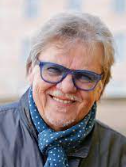
\includegraphics{images/mikko.PNG}}
%    }
%  }
%  \setlength{\fboxsep}{1em}
%  \begin{blackbox}
%  \item}
%  {
%  \end{blackbox}
%  \end{itemize}
%}
\usepackage{awesomebox}
\ifluatex
  \usepackage{selnolig}  % disable illegal ligatures
\fi
\usepackage[]{natbib}
\bibliographystyle{apalike}

\title{TILM 3701 - Tilastotiede ja Data 2022}
\author{Koonneet \and Henri Nyberg\footnote{Turun Yliopisto, matematiikan ja tilastotieteen laitos, \href{mailto:henri.nyberg@utu.fi}{\nolinkurl{henri.nyberg@utu.fi}}} \and Roope Rihtamo\footnote{Turun Yliopisto, matematiikan ja tilastotieteen laitos, \href{mailto:roope.rihtamo@utu.fi}{\nolinkurl{roope.rihtamo@utu.fi}}}}
\date{2022-08-22}

\begin{document}
\maketitle

{
\setcounter{tocdepth}{1}
\tableofcontents
}
\hypertarget{kurssin-rakenne}{%
\chapter*{Kurssin rakenne}\label{kurssin-rakenne}}
\addcontentsline{toc}{chapter}{Kurssin rakenne}

\begin{itemize}
\item
  Tällä kurssilla tarkoituksena on melko yleisellä tasolla johdatella tilastotieteen ja aineistojen (datan) maailmaan pohtimalla myös näiden laajempia merkityksiä tieteellisen tutkimuksen hyvin keskeisinä osina.
\item
  Kurssilla vältetään, mahdollisuuksien mukaan, kovin teknistä matemaattista esitystapaa, mutta tarvittavissa määrin tullaan myös käyttämään tilastotieteen perusopinnoissa tarvittavia matemaattisia merkintöjä ja määritelmiä. Esim. todennäköisyyslaskennan ja tilastollisen päättelyn perusteita ei käydä vielä riittävällä matemaattisella tarkkuudella lävitse, vaan nämä tarkastelut jäävät tätä kurssia seuraavien kurssien (\href{https://opas.peppi.utu.fi/fi/opintojakso/TILM3553/1734?period=2022-2024}{TILM3553 Todennäköisyyslaskennan peruskurssi} tai \href{https://opas.peppi.utu.fi/fi/opintojakso/TILM3568/3385?period=2022-2024}{TILM3568 Todennäköisyyslaskenta sivuaineopiskelijoille} sekä \href{https://opas.peppi.utu.fi/fi/opintojakso/TILM3555/1731?period=2022-2024}{TILM3555 Tilastollisen päättelyn peruskurssi}) asiaksi. Nämä kurssit, yhdessä alkuvaiheen pakollisten matematiikan kurssin lisäksi, muodostavat siis tämän kurssin johdannon kanssa lähtökohdan tilastotieteen opinnoille.
\item
  Luennot eivät suoraan perustu yhteen kirjaan tai lähteeseen. Käytettyjä lähdemateriaaleja luetellaan alapuolella oheislukemiston myötä.
\item
  Oheislukemistoa (sopivilta osin):

  \begin{itemize}
  \tightlist
  \item
    Mellin, I. (2004). Johdatus tilastotieteeseen: Tilastotieteen johdantokurssi (1.kirja). Yliopistopaino, Helsingin yliopisto.
  \item
    Mellin, I. (2000). Johdatus tilastotieteeseen: Tilastotieteen jatkokurssi (2.kirja). Yliopistopaino, Helsingin yliopisto.
  \item
    Mellin, I. (2006). Tilastolliset menetelmät. Luentomoniste, Aalto yliopisto (TKK).
  \item
    Holopainen, M. ja P. Pulkkinen (2008). Tilastolliset menetelmät. Sanoma Pro Oy.
  \item
    Pahkinen, E. ja R. Lehtonen (1989). Otanta-asetelmat ja tilastollinen analyysi. Gaudeamus, Helsinki.
  \item
    Pahkinen, E. ja R. Lehtonen (2004). Practical Methods for Design and Analysis of Complex Surveys. 2. painos, Wiley.
  \item
    Sund, R. (2003). Tilastotiede käytännön tutkimuksessa -kurssi. Helsingin yliopisto.
  \item
    Silver, N. (2014). Signaali ja kohina: Miksi monet ennusteet epäonnistuvat mutta jotkin eivät? Terra Cognita. (Suomentanut Kimmo Pietiläinen)

    \begin{itemize}
    \tightlist
    \item
      Englanninkielinen teos: Silver, N. (2015). The Signal and the Noise: Why So Many Predictions Fail--but Some Don't. Penguin Books; Illustrated edition
    \end{itemize}
  \item
    Pesonen, M. (2017). Kurssimateriaali kurssille Aineistonhankinta ja tutkimusasetelmat, Turun yliopisto.
  \item
    Vartia, Y. (1989). Tilastotieteen perusteet. Yliopistopaino, Helsinki. II painos.
  \end{itemize}
\item
  Muita taustamateriaaleja

  \begin{itemize}
  \tightlist
  \item
    \href{https://tilastokoulu.stat.fi/verkkokoulu_v2.xql?course_id=tkoulu_tilaj\&lesson_id=1\&subject_id=0\&page_type=sisalto}{Tilastokeskuksen tilastokoulu (linkki)}
  \item
    Tilastotieteen sanasto suomi-englanti-suomi, ks. Juha Alho, Elja Arjas, Esa Läärä ja Pekka Pere (2021). \href{https://tilastoseura.fi/}{Tilastotieteen sanasto. Suomen Tilastoseuran julkaisuja 8.}
  \end{itemize}
\end{itemize}

Suuret kiitokset Visa Kuntzelle ja Emil Lehdelle kommenteista ja avusta materiaalin työstämisessä. Kaikki jäljelle jääneet painovirheet ovat materiaalin kokoajien.

\hypertarget{johdantoa-ja-johdattelua-tilastotieteeseen}{%
\chapter{Johdantoa ja johdattelua tilastotieteeseen}\label{johdantoa-ja-johdattelua-tilastotieteeseen}}

\emph{Ihmisellä on luontainen pyrkimys ymmärtää, mitä hänen ympärillään tapahtuu. Ymmärrys perustuu ihmisen tekemiin havaintoihin, joita luokittelemalla tai seuraamalla hän pyrkii löytämään säännönmukaisuuksia. Näiden säännönmukaisuuksien löytäminen vaatii loogisten johtopäätösten tekoa. Pelkän uteliaisuuden tyydyttämiseen ja älyllisen mielihyvän lisäksi ihminen pyrkii ennakoimaan tulevaa ja siten varautumaan tuleviin tapahtumiin\ldots{} Edellä kuvattuja taitoja voi oppia.}

Holopainen ja Pulkkinen, 2008

\hypertarget{tilastotiede-ja-kurssin-idea}{%
\section{Tilastotiede ja kurssin idea}\label{tilastotiede-ja-kurssin-idea}}

\begin{itemize}
\tightlist
\item
  Tämän tilastotieteen ensimmäisen kurssin ideana on (ainakin)

  \begin{itemize}
  \tightlist
  \item
    Esitellä ja johdatella \textbf{tilastolliseen ja tieteelliseen ajatteluun} ja sen hyödyntämiseen eri tyyppisissä tutkimusongelmissa.
  \item
    Esitellä tilastotieteen roolia \textbf{empiirisen tutkimusaineiston keräämisessä ja analyysissä} sekä tarkastella tieteentekemisen ja tilastotieteen suhdetta.
  \item
    Pohtia \textbf{tilastotieteen olemusta tieteenalana} ja tarkastella tilastotieteen ja datatieteiden (data sciencen) samankaltaisuuksia ja eroja.
  \item
    Pohtia \textbf{sattuman ja satunnaisuuden roolia} jokapäiväisessä elämässä ja erityisesti osana tieteellistä tutkimusprosessia.
  \item
    Oppia tilastotieteen peruskäsitteitä ja (tilastollisen) tutkimuksenteon alkeita ja siihen liittyviä mahdollisia ongelmia esimerkiksi tilastollisten aineistojen keräämisessä.
  \item
    Oppia tilastollisten aineistojen \textbf{kuvaamisen ja käsittelyn} alkeita sekä tilasto(tieteellisen)llisen \textbf{mallintamisen} ja \textbf{koeasetelmien} peruskäsitteitä.
  \end{itemize}
\end{itemize}

\vspace{0.75cm}

\begin{itemize}
\tightlist
\item
  Kurssilla käsitellään myös \textbf{tilastollisen päättelyn} peruskäsitteitä ja perusteita kuten

  \begin{itemize}
  \tightlist
  \item
    Mitä on \textbf{todennäköisyys} ja miten sen tulkitaan tilastotieteessä sekä laajemmin tieteessä. Erityisesti tilastotieteen osalta keskiössä on tämän kurssin osalta \textbf{satunnaismuuttujat} sekä niihin liitettävät käsitteet

    \begin{itemize}
    \tightlist
    \item
      \textbf{Odotusarvo}, \textbf{varianssi} ja kahden (tai useamman) satunnaismuuttujan \textbf{korrelaatio}.
    \item
      Satunnaismuuttujien \textbf{todennäköisyysjakaumien} perusteita ja niiden yhteyksiä mm. normaalijakaumaan ja muutamiin muihin keskeisiin jakaumiin.
    \item
      Tilastollinen malli työkaluna satunnaismuuttujien formaalissa mallintamisessa ja päättelyssä. Tilastollisen malliin liittyy (usein) \textbf{parametreja} joihin tilastollinen päättely kohdistuu.
    \item
      Tilastollisten mallien \textbf{estimoinnin} perusidea, eli miten tilastollisen mallin parametreille muodostetaan arvot käytettävissä olevan aineiston pohjalta. Esimerkiksi: mitä tarkoittaa tilastollisen mallin parametrin \textbf{estimaattori} ja sen \textbf{harhattomuus}?
    \item
      Alustavia tarkasteluja tilastollisen mallin uskottavuuden käsitteelle ja \textbf{luottamusväleille} tilastollisen mallin estimoiduille parametreille.
    \end{itemize}
  \end{itemize}
\end{itemize}

\vspace{0.75cm}

\begin{itemize}
\tightlist
\item
  Toinen kurssin keskeisistä teemoista on tarkastella tieteellistä tutkimusprosessia teoriassa ja käytännössä. Tämä sisältää mm. seuraavia aiheita (joita siis käsitellään tällä kurssilla päällisin puolin ja varsin yleisestä näkökulmasta katsoen): tarkemmat yksityiskohdat jäävät tätä kurssia seuraavien tilastotieteen kurssien aihepiireiksi):

  \begin{itemize}
  \tightlist
  \item
    \textbf{Tutkimusongelman} asettaminen: mitä halutaan tutkia?\\
  \item
    Tutkimusongelman täsmentäminen ja \textbf{tutkimusstrategian} laatiminen: millä keinoin asetettuun tutkimusongelmaan voidaan vastata?
  \item
    \textbf{Tutkimusaineiston} (tai vain lyhyemmin \textbf{aineiston} eli \textbf{datan}) kerääminen

    \begin{itemize}
    \tightlist
    \item
      \textbf{Aineiston ennakkoehdot}: mitkä ehdot tulee täyttyä, jotta asetettuun tutkimusongelmaan voidaan vastata?
    \item
      \textbf{Otanta} (ja mittaaminen): miten tutkimusaineisto kerätään niin, että se täyttää aineiston ennakkoehdot? Erilaisissa tutkimuksissa käytetään erilaisia aineistoja kuten:

      \begin{itemize}
      \tightlist
      \item
        Survey- ja rekisteriaineistot
      \item
        Havaintoarvojen välistä korrelaatiota esiintyy mm. aikasarja-aineistojen tai pitkittäisaineistojen tapauksessa
      \end{itemize}
    \end{itemize}
  \end{itemize}
\item
  \textbf{Aineiston kuvaaminen}: minkälaista aineistoa on kerätty ja vastaako se ennakkoehtoja?
\item
  \textbf{Aineiston analyysin} lähtökohtia

  \begin{itemize}
  \tightlist
  \item
    Mitä tilastollista mallia/malleja käytetään?
  \item
    Mitä tarkoitetaan mallien tuntemattomien parametrien arvojen estimoinnilla?
  \item
    Tilastollinen päättely (estimointitulosten pohjalta)
  \end{itemize}
\item
  \textbf{Johtopäätelmien} tekeminen tilastollisen päättelyn pohjalta: saatiinko tutkimusongelmaan vastaus ja kuinka luotettava saatu vastaus on?
\end{itemize}

\hypertarget{tilastotieteen-asema-tutkimusyhteisuxf6n-ulkopuolella}{%
\section{Tilastotieteen asema tutkimusyhteisön ulkopuolella}\label{tilastotieteen-asema-tutkimusyhteisuxf6n-ulkopuolella}}

\begin{itemize}
\tightlist
\item
  Tilastotiede on oppiaineena usein varsin tuntematon toisen asteen opinnoista valmistuneelle, sillä sitä ei juurikaan opeteta lukioissa tai ammattikouluissa huolimatta sen keskeisestä ja kasvavasta roolista tiedemaailman kentillä.
\item
  Tiedeyhteisön ulkopuolellakin \textbf{tilastotiedettä ja tilastotieteilijöitä arvostetaan laajalti}.
\item
  \textbf{Tilastotiede onkin nostanut profiiliaan viimeisten vuosikymmenien aikana} tietoteknisen kehityksen tuotua laajat tietoaineistot ja kehittyneet laskennalliset menetelmät lähes jokaisen kansalaisen saataville.
\item
  Tämä ``datavallankumous'' näkyy tilastotieteilijöiden kysynnässä työmarkkinoilla: erilaisten aineistojen määrän lisääntyessä kasvaa myös kysyntä työntekijöistä, jotka osaavat ammatitaitoisesti käsitellä, tulkita ja mallintaa tilastollisia aineistoja.
\item
  Ei siis liene ihmekään, että erilaisten ``data''-alkuisten työpaikkojen, kuten \textbf{datatieteilijä} (eng. \textbf{data scientist}) tai \textbf{data-analyytikko} ( \textbf{data-analyst}) määrä on kasvanut voimakkaasti jo pidempään. Kaikkia tieto- ja datainensiivisten ammattien tekijöitä yhdistää yksi tekijä: \textbf{heidän tulee hallita ja osata tilastotiedettä!} Karkeistettuna mitä paremmin ja enemmän (laajemmin), sen parempi palkka ja monipuolisemmat työtehtävät!
\end{itemize}

\hypertarget{kurssin-luonne-tilastotieteen-ja-datatieteendata-analytiikan-opintojen-esittelijuxe4nuxe4}{%
\section{Kurssin luonne tilastotieteen (ja datatieteen/data-analytiikan) opintojen esittelijänä}\label{kurssin-luonne-tilastotieteen-ja-datatieteendata-analytiikan-opintojen-esittelijuxe4nuxe4}}

Kurssin mittaan esitellään tilastotieteen perusteiden lisäksi \textbf{miten TY:ssa tilastotieteen opinnoissa syvennytään} tällä kurssilla esiteltäviin menetelmiin, aineistotyyppeihin ja mallinnuskokonaisuuksiin.

\hypertarget{luku2}{%
\chapter{Tieteellinen tieto, tilastot ja arkitieto yhteiskunnassa}\label{luku2}}

\hypertarget{alaluku21}{%
\section{Mitä on tiede?}\label{alaluku21}}

\hypertarget{alaluku22}{%
\section{Tieteellinen menetelmä}\label{alaluku22}}

\hypertarget{alaluku23}{%
\section{Tilastojen yleisestä roolista yhteiskunnassa}\label{alaluku23}}

\hypertarget{alaluku24}{%
\section{Mitä on tutkimus?}\label{alaluku24}}

\hypertarget{alaluku25}{%
\section{Tieteellisen tutkimuksen vaiheet ja tulosten julkaiseminen}\label{alaluku25}}

\hypertarget{tilastotiede-tieteenalana}{%
\chapter{Tilastotiede tieteenalana}\label{tilastotiede-tieteenalana}}

Tässä luvussa hahmottelemme tilastotieteen piirteitä tieteenalana. Käymme läpi tilastotieteelle
ominaisia piirteitä, jotka erottavat sen niin lähitieteistä, kuten matematiikasta ja tietojenkäsit-
telytieteestä, kuin myös sovellusaloista. Usein näkee tilastotieteen typistettävän vain työkaluksi
eri sovellusalojen empiiriseen tutkimukseen siitäkin huolimatta että tilastotieteellä on oma rikas
teoriapohjansa sekä kiistaton asema omana tieteenalanaan.
Tieteenalan määritteleminen lyhyesti on aina hieman hankalaa. Tästä huolimatta seuraavassa
yritämme osaltaan vastata seuraaviin kysymyksiin:

\begin{itemize}
\tightlist
\item
  Mitä tilastotiede on ja mitä se ei ole? Miksi tilastotiede ei ole vain sovellettua matematiikkaa
  tai matematiikalla höystettyä tietojenkäsittelyä?
\item
  Mihin tilastotiedettä käytetään? Onko tilastotieteellä käyttöä ns. ``akatemian'' eli tutki-
  musyhteisön ulkopuolella?
\item
  Tilastotieteelle tyypillistä kritiikkiä?
\end{itemize}

\hypertarget{lisuxe4uxe4-tilastotieteen-perustermejuxe4}{%
\section{Lisää tilastotieteen perustermejä}\label{lisuxe4uxe4-tilastotieteen-perustermejuxe4}}

Seuraavia tilastotieteen esittelyä ja karakterisointeja ajatellen määritellään seuraavassa lisää tilastotieteellisen tutkimuksen peruskäsitteitä. Näihin käsitteisiin paneudutaan osaltaan tarkemmin mm. luvussa ?? {[}otantaluku{]}.

\begin{itemize}
\tightlist
\item
  Tilastotieteellinen tutkimus tarkastelee reaalimaailman ilmiöitä. Täten tutkimuskohteena on tavallisessa elämässä tavattavia asioita, ihmisiä tai tapahtumia. Tutkimuskohteita kutsutaan tilastoyksiköiksi ja niiden joukkoa kutsutaan populaatioksi (perusjoukoksi). Esimerkiksi jos tutkitaan kuntavaaleissa äänestävien tuloja niin jokainen äänestysikäinen muodostaa oman tilastoyksikkönsä (ks. alla) ja täten populaationa (perusjoukkona) toimii kaikki
  äänestysikäiset kansalaiset. Jos taas tutkitaan äänestysaktiivisuutta eri kunnissa, muodostaa jokainen kunta oman tilastoyksikkönsä ja kaikki Suomen kunnat muodostavat populaation.
\end{itemize}

\begin{noteblock}{}
\textbf{Populaatio}

Konkreettinen tai hypoteettinen tutkimuskohteiden joukko, joka
koostuu kaikista tilastoyksiköistä

\end{noteblock}

\begin{itemize}
\item
  Populaation muodostavilta tilastoyksiköiltä tarkastellaan niiden ominaisuuksia, eli \textbf{tilastollisia muuttujia}. Edellisissä esimerkeissä nämä olisivat esim. äänestäjien tulot ja kuntien äänestysprosentti. Mielenkiinnon kohteena olevia tilastollisia muuttujia kutsutaan \textbf{tutkimusmuuttujiksi} (tulot ja kuntien äänestysprosentti) ja niiden lisäksi voidaan kerätä ylimääräistä tietoa eli \textbf{taustamuuttujia} (näitä voisi olla esimerkiksi asuinpaikka ja kunnan väkiluku).
\item
  Tilastoyksiköiden tilastollisilla muuttujilla on tietty mahdollisten arvojen joukko, ja näillä arvoilla on jokin \textbf{jakauma} populaatiossa. Esimerkiksi tulot voivat määritelmästä riippuen saada minkä tahansa positiivisen arvon mutta äänestysprosentti on luonnollisesti rajattu nollan ja sadan prosentin väliin.
\end{itemize}

\begin{noteblock}{}
\textbf{Tilastoyksikkö ja tilastollinen muuttuja}

Populaation muodostavilta tilastoyksiköiltä (populaation alkioilta) tarkastellaan tilastollisia muuttujia, joita voidaan mitata tai havaita.

\end{noteblock}

\begin{itemize}
\tightlist
\item
  Kun tarkasteltavien tilastoyksikön tilastollisten muuttujien (numeeriset) arvot havaitaan, kutsutaan näiden arvojen joukkoa \textbf{havainnoksi}
\end{itemize}

\begin{noteblock}{}
\textbf{Havainto}

Havainto muodostuu tilastoyksikön tarkasteltavien tilastollisten muuttujien havaitusta arvoista.

\end{noteblock}

\begin{itemize}
\item
  Populaatio koostuu tilastoyksiköistä, joilla on tilastollisia muuttujia. Tarkasteltavista tilastollisista muuttujista kerätään havaintoja, joiden pohjalta tutkitaan \textbf{populaation ominaisuuksia}.
\item
  Kerättyjen havaintojen joukko muodostaa \textbf{havaintoaineiston}, eli \textbf{datan}.
\end{itemize}

\begin{noteblock}{}
\textbf{Havaintoaineisto/data}

Havaintoaineisto, data, on tilastoyksiköiden tilastollisista muuttujista kerätty havaintojen joukko.

\end{noteblock}

\textbf{Tiivistettynä}:

\begin{itemize}
\tightlist
\item
  Populaatio tutkimuksen kohteena olevia tilastoyksiköitä.
\item
  Havaitaan tilastoyksiköistä tutkimuksen kannalta mielenkiintoisia tilastollisten muuttujien numeerisia arvoja.
\item
  Nämä havainnot muodostavat havaintoaineiston, eli datan, jota voidaan käyttää tutkimuksessa.
\end{itemize}

-- Terminologiaa (käydään vielä läpi tarkemmin jatkossa):
- Tilastoala = Tilastotiede + Tilastotoimi
- Tilastotiede = Teoreettinen tilastotiede + Soveltava tilastotiede
- Tilastotoimi = Tilastojen tuotanto + Tilastojen hyödyntäminen

\hypertarget{mituxe4-tilastotiede-on-ja-mituxe4-se-ei-ole}{%
\section{Mitä tilastotiede on ja mitä se ei ole?}\label{mituxe4-tilastotiede-on-ja-mituxe4-se-ei-ole}}

\begin{itemize}
\tightlist
\item
  Aloitetaan tarkastelemalla erinäisiä \textbf{tilastotieteen ``karakterisointeja''} eri tahojen ja tutkijoiden toimesta:

  \begin{itemize}
  \tightlist
  \item
    \textbf{\emph{Tilastotiede on tietotuotannon teknologiaa}}, \emph{jonka avulla voidaan suorittaa kvantitatiivisten tietojen joukkotuotantoa ja havaintoihin perustuvia tieteellisiä ja käytännöllisiä päätöksiä. Tilastotiede on siis yksikköjen muodostamaan joukkoon liittyvän numeerisen tietoaineiston keräämistä, analysointia ja tulkintaa koskeva tiede} \footnote{\href{https://fi.wikipedia.org/wiki/Leo_T\%C3\%B6rnqvist}{Leo Törnqvistin}, Suomen ensimmäisen tilastotieteen professorin, esittämä luonnehdinta (Vartia, 1989).}.
  \item
    \textbf{\emph{Tilastotiede on yleinen menetelmätiede}}, \emph{jota sovelletaan, jos reaalimaailman ilmiöstä halutaan tehdä johtopäätöksiä ilmiötä kuvaavien kvantitatiivisten tai numeeristen tietojen perusteella sellaisissa tilanteissa, joissa tietoihin liittyy epävarmuutta tai satunnaisuutta} \footnote{Mellin, (2005).}.
  \item
    \textbf{\emph{Tilastotiede on yleinen menetelmätiede}}, \emph{jota sovelletaan, jos reaalimaailman ilmiöstä halutaan tehdä johtopäätöksiä ilmiötä kuvaavien kvantitatiivisten tai numeeristen tietojen perusteella sellaisissa tilanteissa, joissa tietoihin liittyy epävarmuutta tai satunnaisuutta.}
  \item
    \emph{Vale, emävale, tilasto} \footnote{\href{https://fi.wikipedia.org/wiki/Mark_Twain}{Mark Twain} popularisoi tämän lausahduksen teoksessaan \emph{Chapters from My Autobiography} jo vuonna 1907.}.
  \item
    \emph{Statistics concerns what can be learned from data} \footnote{(A.C. Davison)}.
  \item
    \emph{``Maalaisjärjen tehostamista''} \footnote{(Sund, 2003)}.
  \end{itemize}
\item
  Tilastotiede siis \textbf{kehittää} ja \textbf{soveltaa menetelmiä} ja (tilastollisia) \textbf{malleja}, joiden avulla reaalimaailman ilmiöistä voidaan tehdä johtopäätöksiä ilmiöitä kuvaavien numeeristen tai kvantitatiivisten tietojen perusteella tilanteissa, joissa tietoihin liittyy \textbf{epävarmuutta ja satunnaisuutta}.

  \begin{itemize}
  \tightlist
  \item
    Tilastollisten menetelmien avulla pyritään löytämään reaalimaailman satunnaisia ilmiöitä kuvaavista numeerisista (eli kvantitatiivisista) tiedoista \textbf{systemaattisia piirteitä} joita jalostetaan sellaiseen muotoon, että ilmiöistä voidaan tehdä päätelmiä.

    \begin{itemize}
    \tightlist
    \item
      Vrt. signaalin ja kohinan erottaminen (ks. Silver, 2014).
    \end{itemize}
  \item
    Tilastolliset mallit perustuvat todennäköisyyslaskentaan ja niillä mallinnetaan reaalielämän ilmiöiden alla piileviä prosesseja tai mekanismeja. Näiden prosessien tuottamia tietoja (aineistoja) tiivistetään usein graafisiksi esityksiksi ja tunnusluvuiksi sekä tilastollisten mallien parametreiksi, joiden pohjalta johtopäätöksiä tehdään.
  \item
    Tässä onnistuakseen tilastollisten menetelmien tuleekin pyrkiä erottelemaan \textbf{sattuma} ja \textbf{systemaattisuus} tarkasteltavissa ilmiöissä tai, tarkemmin, niitä kuvaavissa aineistoissa, jotta johtopäätökset olisivat luotettavia.
  \end{itemize}
\end{itemize}

\textbf{Voidaan sanoa, että saadakseen tarkemmin selville mitä tilastotiede on, pitää opiskella tilastotiedettä ja sen käyttöä!}

\begin{itemize}
\item
  Edellisten tilastotieteen yleismaailmallisten luonnehdintojen jälkeen onkin sopivaa kysyä \textbf{mitä tilastotiede ei ole}.

  \begin{itemize}
  \tightlist
  \item
    Vaikka sana \textbf{tilasto} tuo useimmille ensimmäisenä mieleen yhteiskuntaa ja sen toimintaa kuvaavat \textbf{numeeristen tietojen järjestelmälliset kokoelmat}, tilastotiede ei suinkaan ole ainoastaan tilastojen ja niiden tekemisen oppia.

    \begin{itemize}
    \tightlist
    \item
      Tämä siitäkin huolimatta, että niiden menetelmien konstruointi, joilla näitä tilastoja tuotetaan, jalostetaan ja analysoidaan on keskeinen osa tilastotiedettä. Tilastot ovat siis usein tilastotieteen soveltajan tutkimuskohteena ja tilastojen laadinnassa käytetään apuna tilastotieteen menetelmiä.
    \item
      Suomessa \href{https://www.stat.fi/}{Tilastokeskus} toimii virallisena tilastoviranomaisena ja tilastotuottajana. Tätä \textbf{tilastotuotannon} kokonaisuutta nimitetään ajoittain \textbf{tilastotoimeksi}. \textbf{Tilastotieteen käyttöalue on paljon tätä laajempi}.
    \end{itemize}
  \item
    Tilastotieteen kannalta mikä tahansa reaalimaailman ilmiötä kuvaava \textbf{numeeristen tai kvantitatiivisten tietojen järjestelmällinen kokoelma} voi muodostaa \textbf{tilastollisen aineiston} ja siten tilastollisen tutkimuksen mahdollisen kohteen.
  \item
    Esimerkiksi kaikki \textbf{empiirisen} tai \textbf{kvantitatiivisen}
    tutkimuksen tutkimus- tai havaintoaineistot ovat tilastotieteen kannalta tilastollisia aineistoja.
  \end{itemize}
\item
  Tilastotiede sijoittuu tieteiden kentässä matematiikan, filosofian ja tietojenkäsittelytieteen rinnalle. Tästä huolimatta se ei kuitenkaan ole yksiselitteisesti minkään näiden osa-alue.

  \begin{itemize}
  \tightlist
  \item
    \textbf{Tilastotiede ei ole matematiikan osa-alue}, sillä tilastotiede lähestyy tieteellistä ongelmanratkaisua eri tavoin: matematiikka on tietyllä tavallaan aina eksaktia ja sen tulokset perustuvat formaaliin deduktioon ja loogisiin todistuksiin, johtaen usein ``eksaktiin'\,' ratkaisuun tai matemaattisesti formaaliin ratkaisun esitystapaan. Tilastotiede sen sijaan on aina konteksti- ja aineistopohjaista ja perustuu induktiiviseen päättelyyn. Saadut tulokset ovat aina epävarmoja - koska ne kuvailevat epävarmaa tietoa generoivia prosesseja!

    \begin{itemize}
    \tightlist
    \item
      Tilastotiede on siis hyvä nähdä omana tieteenalanaan matemaattisesta esitystavastaan huolimatta. Eihän esimerkiksi myöskään fysiikkaa (sentään) pidetä matematiikan osa-alueena!
    \end{itemize}
  \item
    \textbf{Tilastotiede ei ole myöskään tietojenkäsittelytieteen osa-alue}, vaikkakin useiden laskennallisten menetelmien ja tehokkaan tietojenkäsittelyn rooli tilastollisissa analyyseissä on jatkuvasti kasvanut. Tietojenkäsittelytieteen teoria ei rakennu tilastotieteen tavoin ajatukselle epävarmoista ja satunnaisista reaalimaailman ilmiöistä.
  \item
    Vaikka nämä ja jotkin muut alat jakavat tilastotieteen kanssa useita piirteitä ja ominaisuuksia, on tilastotiede kuitenkin siis perustellusti oma tieteenalansa. Tämä erottelun vaikeus jo itsessään todistaa kuinka keskeinen rooli tilastotieteellä on eri aloilla!
  \end{itemize}
\item
  Tilastotiede ei siis kuulu yksiselitteisesti sen lähitietieden alle, vaan muodostaa oman tieteenalan omine teorioineen ja tieteellisine premisseineen. Käsittelemme myöhemmin tilastotieteen roolia matematiikan ja/tai datatieteiden (``data science'') kokonaisuudessa ja keskustelemme tarkemmin näiden erojen luonteesta.
\item
  \textbf{Tilastotiede yleisenä menetelmätieteenä}

  \begin{itemize}
  \tightlist
  \item
    Tieteellistä tietoa ympäröivästä maailmasta hankitaan tieteellisillä \textbf{menetelmillä/metodeilla} (Ks. tieteellisen menetelmän kriteerit {[}Luku ?? 2{]})), joiden avulla tutkitaan jotain ilmiötä tai sen generoimaa kvantitatiivista mutta epävarmaa tietoa sisältävää aineistoa.
  \item
    Tilastotieteessä kehitetyt ja kehitettävät menetelmät antavat tutkijoille yhtenevät ja tiedeyhteisön hyväksymät raamit, jotka mahdollistavat (tilastollisen) päättelyn ja päätöksenteon epävarman tiedon vallitessa. Näin voidaan uskottavasti ja luotettavasti tiivistää tietoa, jota erilaiset aineistot sisältävät, perustaa johtopäätöksiä näille tiivistyksille ja saavuttaa uusia tieteellisiä löytöjä.

    \begin{itemize}
    \tightlist
    \item
      Tilastotieteen menetelmien käyttö ja soveltaminen onkin siis aina alakohtaista. Tästä huolimatta tilastollisia menetelmiä sovelletaan aina johonkin \textbf{aineistoon}!
    \end{itemize}
  \item
    Tilastotieteen nähdäänkin usein kuuluvan ns. \textbf{menetelmätieteisiin}, joissa mm.:

    \begin{itemize}
    \tightlist
    \item
      Kehitetään työkaluja muiden tieteiden tutkimusongelmien ratkaisuksi
    \item
      On myös oma sovelluksista vapaa teorianmuodostuksensa
    \end{itemize}
  \item
    Menetelmäkehityksen näkökulma tilastotieteeseen: \emph{tilastotiede kehittää matemaattisia} \textbf{\emph{malleja}} \emph{satunnaisilmiöitä kuvaavia kvantitatiivisia tietoja generoiville prosesseille.} Koska tietoihin liittyy \textbf{epävarmuutta} tai \textbf{satunnaisuutta}, \textbf{tilastolliset mallit} perustuvat \textbf{todennäköisyyslaskentaan}.
  \item
    Juuri sattuman ja epävarmuuden huomioiminen tutkimusasetelmissa erottaa tilastotieteen muista menetelmätieteistä!
  \end{itemize}
\item
  \textbf{Aineisto:} Tilastotieteessä lähtökohtana ja ratkaisevassa asemassa on siis aina jonkin satunnaisilmiön generoima aineisto, josta haluamme oppia tai tietää lisää, kenties voidaksemme tehdä suuria yhteiskunnallisia päätöksiä sen pohjalta!

  \begin{itemize}
  \tightlist
  \item
    Tämä aineistokeskeisyys osaltaan erottaa tilastotieteen rajatieteistään ja osaltaan tuo sen lähemmäksi niitä ja sovellusalojaan. (Näitä tarkastellaan myöhemmin luvussa ?.?).
  \item
    Aineistoa analysoidaan, kuvaillaan ja mallinnetaan tilastollisin menetelmin, joiden kehittäminen on keskeinen osa tilastotiedettä.
  \item
    Pelkkä menetelmien kehittäminen kuuluu pitkälti matemaattisen tai teoreettisen tilastotieteen osa-alueelle.
  \item
    Pelkkä ainestoon keskittyminen ja (mekaaninen) analysointi voi sen sijaan olla joissain tilanteissa pitkälti tietojenkäsittelyä.
  \item
    \textbf{Tilastollinen ``mallintaminen''} löytyykin näiden välistä ja se sisältää eri alojen sovelluksista kumpuavan tarpeen uusien menetelmien kehittämiseen.

    \begin{itemize}
    \tightlist
    \item
      Tämä vuoropuhelu muodostaa tilastotieteelle luonnollisen ``takaisinkytkennän'' teoreettisen ja soveltavan puolen välillä: uudet teoreettiset menetelmät vastaavat soveltavan tilastotieteen ongelmiin mutta herättävät aina uusia kysymyksiä, jotka palautuvat taas teoreetikon pöydälle!
    \end{itemize}
  \item
    Luonnollisesti valtaosa tilastotieteilijöistä ja lähitieteiden harrastajista asettuvat näiden äärimmäisten luonnehdintojen välimaastoon eikä tarkkaa luokittelua ole sinänsä tarpeen tehdä ja korostaa.
  \item
    Joka tapauksessa tilastotieteen kehityksen keskiössä ovat aina sovellusalakohtaiset ongelmat, joista useat palautuvat yleisemmälle tasolle teoreettisen tilastotieteen kehityspolkuihin.
  \end{itemize}
\end{itemize}

\hypertarget{tilastotieteen-suhde-matematiikkaan-tietojenkuxe4sittelytieteeseen-ja-datatieteeseen-data-science}{%
\section{Tilastotieteen suhde matematiikkaan, tietojenkäsittelytieteeseen ja datatieteeseen (data science)}\label{tilastotieteen-suhde-matematiikkaan-tietojenkuxe4sittelytieteeseen-ja-datatieteeseen-data-science}}

\hypertarget{luku4}{%
\chapter{Sattuma ja satunnaisuus}\label{luku4}}

\hypertarget{alaluku41}{%
\section{Satunnaisilmiöt ja satunnaismuuttujat tilastotieteessä}\label{alaluku41}}

\hypertarget{alaluku42}{%
\section{Tilastotieteen suhde satunnaisuuteen ja todennäköisyyksiin}\label{alaluku42}}

\hypertarget{alaluku43}{%
\section{Tilastolliset mallit, jakaumat ja parametrit}\label{alaluku43}}

\hypertarget{alaluku44}{%
\section{Odotusarvo ja varianssi}\label{alaluku44}}

\hypertarget{alaluku45}{%
\section{Joitain jakaumia}\label{alaluku45}}

\hypertarget{normaalijakauma}{%
\subsection{Normaalijakauma}\label{normaalijakauma}}

\hypertarget{bernoulli--binomi--ja-poisson-jakauma}{%
\subsection{Bernoulli-, binomi- ja Poisson-jakauma}\label{bernoulli--binomi--ja-poisson-jakauma}}

\hypertarget{alaluku46}{%
\section{Sattuman rooli tieteenteossa: Vale-emävale-tilasto?}\label{alaluku46}}

\hypertarget{luku5}{%
\chapter{Tilastolliset aineistot, niiden kerääminen ja mittaaminen}\label{luku5}}

Edellisessä luvussa käsiteltiin tilastotieteen suhtautumista satunnaisilmiöihin. Tässä luvussa tarkastelemme lähemmin miten reaalimaailman satunnaisilmiöistä kerätään tietoa ja miten niitä voidaan mitata. Tilastotieteen perusoppimäärä rakentuu ajatukselle ilmiöiden tutkimisesta rajallisen ja epävarman tiedon vallitessa. Käytännössä tämä tarkoittaa sitä, että tutkimuksen kohteena olevat rajalliset aineistot sisältävät niin systemaattista kuin satunnaisuudesta johtuvaa vaihtelua. Tilastollisten menetelmien avulla pyrimme erottamaan systemaattisen vaihtelun satunnaisesta sekä tekemään tilastollista päättelyä aineiston generoimasta mekanismista. Lyhyesti tämä tarkoittaa aineiston systemaattisen vaihtelun tilastollista mallintamista ja sen parametrien estimointia otoksesta, joka kattaa vain (pienen) osajoukon koko populaation (perusjoukon) tilastoyksiköistä.

Voidaksemme tehdä uskottavaa päättelyä ``havainnoista parametreihin'', tulee otoksen olla riittävän \textbf{edustava}. Tämän luvun keskeisin oppi onkin, että miten otanta tulisi suorittaa, jotta havaintoaineisto olisi \textbf{edustava otos} populaatiosta, silloin kun aineisto kerätään otannalla. Vaikka aineiston hankinta vaatii yleensä runsaasti käytännön työtä, kannattaa se tehdä huolellisesti, sillä huonosti toteutetun otannan vuoksi tutkimusongelman kannalta keskeisiä johtopäätöksiä ei voida tehdä!

\hypertarget{alaluku51}{%
\section{Kertausta: Data eli aineisto}\label{alaluku51}}

\begin{itemize}
\item
  \textbf{Tilastollinen tutkimus} aloitetaan tutkimusaineiston keruun suunnittelulla.
\item
  Kertauksen vuoksi: tilastollinen tutkimusaineisto (havaintoaineisto) kostuu tilastoyksiköiden populaatiosta havaituista tilastoyksiköiden muuttujien arvoista.
\item
  Havaintoaineisto voidaan koota taulukoksi, johon listataan tilastoyksiköt riveille ja tilastomuuttujat sarakkeisiin. Jos havaintoaineisto koostuu \(n\) tilastoyksiköstä, joista jokaisesta on kerätty esim. \(m\) tilastomuuttujasta havainnot, niin havainnot voidaan kirjoittaa taulukon muotoon
\end{itemize}

\begin{longtable}[]{@{}lllll@{}}
\toprule
& tilastomuuttuja 1 & tilastomuuttuja 2 & \ldots{} & tilastomuuttuja \(m\) \\
\midrule
\endhead
tilastoyksikkö 1 & \(x_{1,1}\) & \(x_{1,2}\) & & \(x_{1,m}\) \\
tilastoyksikkö 2 & \(x_{2,2}\) & \(x_{2,2}\) & & \(x_{2,m}\) \\
\ldots{} & \ldots{} & \ldots{} & \ldots{} & \\
tilastoyksikkö \(n\) & \(x_{n,1}\) & \(x_{1,2}\) & & \(x_{n,m}\) \\
\bottomrule
\end{longtable}

Tässä siis rivillä \(i\) on \(i\). \textbf{tilastoyksikön} havainto ja \(j\) sarakkeessa on \(j\). tilastollisesta muuttujasta havaitut arvot \(x_{i,j}\). Ts. yhdellä rivillä on yhden tilastoyksikön tiedot kaikista tilastomuuttujista ja yksi sarake on kaikkien tilastoyksiköiden tiedot yhdestä tilastomuuttujasta.

\begin{itemize}
\tightlist
\item
  Usein (varsinkin parhaillaan kiihtyvällä vauhdilla) kerättävät havaintoaineistot ovat niin suuria, ettei edellisenkaltaisesta havaintotaulukosta voida usein suoraan tarkastelemalla nähdä aineiston pääpiirteitä.

  \begin{itemize}
  \tightlist
  \item
    Tällöin on tarpeen luokitella aineistoa taulukon muodostamiseksi.\\
  \item
    Luokittelussa on kysymys aineiston tiivistämisestä kohtuullisen kokoiseksi ja havainnollisempaan muotoon. Luokittelussa tilastomuuttujan arvot sijoitetaan eri luokkiin siten, että yhden tilastomuuttujan arvo voi kuulua vain yhteen luokkaan. Luokka ilmoitetaan yleensä luokkavälinä, kuten reaalilukuvälinä. Esimerkiksi henkilön ikä on tapana luokitella ikäjakauman kuvaamisessa 10-vuotisluokkiin (15-24, 25-34, \ldots), vaikka periaatteessa ikä voitaisiin ilmoittaa minuutinkin tarkkuudella.\\
  \item
    Luokkien lukumäärään vaikuttavat muun muassa tilastomuuttujan arvojen vaihteluväli ja havaintoaineiston laajuus. Luokittelussa pyritään siihen, että luokkien lukumäärä saadaan tarvittaessa luokkia yhdistämällä kohtuulliseksi ja että luokat valitaan tasavälisesti eli siten, että kahden peräkkäisen luokan alarajojen erotus on vakio. Kun aineistoa luokitellaan, aineiston luettavuus paranee mutta toisaalta osa tiedoista menetetään eivätkä yksittäiset havaintoarvot ole enää tiedossa.\\
  \item
    Emme vielä tällä kurssilla etene tämän pidemmälle tilastografiikan esittämisessä ja siihen liittyvissä pohdinnoissa. Muun muassa tilastollisen päättelyn peruskurssi (TILM3555) vastaa näihin kysymyksiin tarkemmin. Graafiset menetelmät ovat joka tapauksessa erittäin tärkeä osa aineiston havainnollistamista. Kuvat helpottavat aineiston tulkitsemista ja toimivat usein perusteltuna lähtökohtana monimutkaisempien tilastollisten mallien (ja algoritmien) sovittamiselle.
  \end{itemize}
\item
  Kvantitatiivisen tutkimuksen aineistoksi kelpaa periaatteessa kaikki havaintoihin perustuva informaatio, joka on \textbf{mittauksen} avulla muutettavissa numeeriseen muotoon.

  \begin{itemize}
  \tightlist
  \item
    Havaintoyksiköiden tilastollisten muuttujien numeerisia arvoja kutsutaan \textbf{havaintoarvoiksi} tai \textbf{havainnoiksi}.
  \item
    Kaikki havaitut tilastolliset muuttujat eivät ole aina mielenkiintoisia. Tutkimuksen kannalta mielenkiintoisia muuttujia kutsutaan \textbf{tutkimusmuuttujiksi}, joiden lisäksi havaintoaineisto pitää mahdollisesti sisällään \textbf{taustamuuttujia}.

    \begin{itemize}
    \tightlist
    \item
      Esimerkiksi, jos tutkimuksella halutaan tietoa suomalaisen aikuisväestön mielipiteistä, havaintoyksikköinä ovat aikuisväestöön kuuluvat henkilöt. Jos halutaan tietoa suomalaisista kunnista, havaintoyksikköinä ovat Suomen kunnat jne.
    \item
      Ensimmäisessä tapauksessa tilastollisina muuttujina on aikuisväestön mielipiteet, joita voidaan selvittää esimerkiksi kyselytutkimuksella. Toisaalta voidaan myös kerätä taustamuuttujiksi haastatelluista muita tietoja, kuten asuinpaikka, ikä ja ammatti.
    \end{itemize}
  \item
    Kaikkia mielenkiintoisia muuttujia ei kuitenkaan välttämättä voida havaita, eli niille ei voida määrittää numeerista arvoa.
  \item
    Tällöin puhutaan nk. \textbf{latenteista muuttujista}, eli muuttujista joita ei suoraan havaita mutta joiden oletetaan vaikuttavan havaittavien muuttujien taustalla. Latentteja muuttujia voidaan rakentaa tilastollisten mallien avulla käyttäen hyödyksi niihin liittyviä havaittuja muuttujia.
  \item
    Latentteja muuttujia ovat esimerkiksi elämänlaatu, onnellisuus, konservatiivisuus, yms.
  \end{itemize}
\item
  Tilastollinen tutkimus voi olla joko \textbf{kokonaistutkimus} tai \textbf{otantatutkimus}.

  \begin{itemize}
  \tightlist
  \item
    \textbf{Kokonaistutkimuksessa} tutkitaan kaikkia ajateltavissa olevia kohteita (kaikki perusjoukon alkiot tutkitaan).

    \begin{itemize}
    \tightlist
    \item
      Esimerkiksi jos tutkitaan Suomen kuntia, niin kokonaistutkimuksessa tutkitaan kaikki kunnat.
    \item
      Tai jos tutkitaan jonkin lääkeaineen vaikutuksia ihmisiin, niin tutkitaan jokainen ihminen erikseen. Selvää on, että tällainen kokonaistutkimus olisi liian vaikeaa toteuttaa.
    \end{itemize}
  \item
    \textbf{Otantatutkimuksessa} tutkimus kohdistetaan johonkin (populaation/perusjoukon) osajoukkoon ja johtopäätelmiä populaatiosta/perusjoukosta tehdään otokseen perustuen.

    \begin{itemize}
    \tightlist
    \item
      Perusjoukosta otokseen poimittuja alkioita kutsutaan \textbf{otosyksiköiksi} ja niiden muodostama osajoukko, eli \textbf{otos}, on se osa perusjoukkoa, joka tutkitaan tutkimusaineiston keräämisen jälkeen.
    \item
      Lääketutkimusta tehdäänkin poikkeuksetta otantatutkimuksena (ja kontrolloituina kokeina, ks. alempaa), jolloin lääkettä testataan vain osajoukolla koko ihmispopulaatiosta ja tämän osajoukon alkiot ovat otosyksiköitä.
    \item
      Näin toimimalla, ja riittävän edustavalla otoksella, saadaan kuitenkin tarpeeksi tietoa lääkeaineen vaikutuksista ja tulokset voidaan yleistää populaatiotasolle ja lääke ottaa käyttöön.
    \item
      Otantatutkimus on halvempi kuin kokonaistutkimus ja tulokset saadaan nopeammin!
    \end{itemize}
  \end{itemize}
\item
  Usein on kuitenkin niin, että koko populaation tutkiminen ei ole mahdollista tai kannattavaa. Tällöin tehtävä tutkimus on otantatutkimus ja tutkittavaksi valitaan perusjoukon osajoukko sopivaa \textbf{otantamenetelmää} (ks. alaluku \ref{alaluku55}) käyttäen.

  \begin{itemize}
  \tightlist
  \item
    Esimerkkinä aseiden patruunoita valmistava tehtailija, joka haluaisi tutkia toimivatko kaikki ammukset tai kaikkien suomalaisten haastatteleminen suomalaisten mielipiteitä kartoitettaessa. Myöskään valaisimien valmistaja tuskin tekee kokonaistutkimuksia valmistamiensa tuotteiden kestoajan selvittämiseksi.
  \end{itemize}
\item
  Tämän vuoksi useimmiten keskitytään perusjoukkoa edustavan pienemmän, mieluusti satunnaisesti valitun osajoukon eli \textbf{otoksen} tutkimiseen.

  \begin{itemize}
  \tightlist
  \item
    Otantatutkimuksissa tiedot kerätään useimmiten haastattelemella, kirjallisella/sähköisellä kyselyllä tai suoraan tietorekistereistä. Tiedonkeruun toteuttaminen (eri sovelluksissa) määrää osaltaan käytettävän otantamenetelmän.
  \item
    Teoriassa äärelliseen perusjoukkoon kohdistuvat kokonaistutkimukset voidaan aina tulkita otantatutkimuksiksi (perusjoukko tulkitaan otokseksi hypoteettisesta äärettömästä perusjoukosta)!

    \begin{itemize}
    \tightlist
    \item
      Esimerkiksi Galilein tekemät painovoiman vaikutusta kappaleiden putoamisaikaan liittyneet mittaukset. Koetuloksia (mittauksia) voidaan pitää otoksena äärettömästä mahdollisten koetulosten joukosta. Tällöin ainoa mahdollisuus ilmiön tutkimiseen on käyttää otantaa.
    \end{itemize}
  \end{itemize}
\item
  Otantatutkimuksen tulokset voivat olla luotettavampia kuin kokonaistutkimuksen.

  \begin{itemize}
  \tightlist
  \item
    Otantatutkimuksessa voidaan panostaa enemmän huolelliseen ja tarkkaan mittaamiseen sekä valitun otoksen tavoittamiseen.
  \item
    Kokonaistutkimuksessa vastauskato ja tarkasteltavan populaation valintavirhe ovat mahdollisia siinä kuin otantatutkimuksessakin.
  \end{itemize}
\item
  Otantateoria on yksi tilastotieteen keskeisimpiä oppeja ja tarjoaa teoreettisen kehikon empiiristen tutkimusten tulosten yleistämiseen. Tarkastellaan siis tarkemmin otannan ideaa ja toteuttamista seuraavassa alaluvussa.
\end{itemize}

\hypertarget{alaluku52}{%
\section{Otannan idea}\label{alaluku52}}

\begin{itemize}
\tightlist
\item
  Otantatutkimuksen (karkeat) suunnittelu- ja työvaiheet ovat seuraavat:

  \begin{enumerate}
  \def\labelenumi{\arabic{enumi}.}
  \tightlist
  \item
    Tavoitteiden asettaminen
  \item
    Perusjoukon (populaation) asettaminen
  \item
    Kehikko
  \item
    Kerättävän informaation sisältö (mitä tietoa todella tarvitaan, mitä voidaan jättää pois, suunnitellaan kysymykset ja mahdollinen kyselylomake)
  \item
    Otoskoon määrittäminen
  \item
    Suoritetaan otoksen poiminta, tietojen keräys ja tarkastus
  \item
    Aineiston taulukointi ja analysointi
  \item
    Raportin laatiminen
  \end{enumerate}
\item
  Otantatutkimuksessa ajatuksena on siis poimia \textbf{edustava otos} siitä populaatiosta (perusjoukosta), joka on mielenkiinnon kohteena eli jota halutaan tutkia ja josta halutaan tietoja.

  \begin{itemize}
  \tightlist
  \item
    \textbf{Tavoiteperusjoukko} on joukko, johon otannan myötä saatavat tutkimustulokset halutaan yleistää. Toisin sanoen, se mistä haluamme tietoja määrää populaation.
  \end{itemize}
\item
  \textbf{Kohdeperusjoukko} on joukko, jota koskevia tietoja halutaan kerätä.

  \begin{itemize}
  \tightlist
  \item
    Esimerkiksi äänestysikäiset Suomen kansalaiset.
  \item
    Usein tavoiteperusjoukko = kohdeperusjoukko.
  \item
    Tavoiteperusjoukko voi joskus olla laajempi (esim. `'ihmiset'' vs.~`'suomalaiset'').
  \end{itemize}
\item
  Tutkimuksessa (edustavaan) otokseen poimitut tilastoyksiköt, näiden tilastolliset muuttujat ja niiden arvot muodostavat \textbf{otosaineiston} eli siis tutkimus- tai havaintoaineiston (datan).

  \begin{itemize}
  \tightlist
  \item
    Tutkimuskysymykseen vastatakseen tutkija valitsee sopivan tilastollisen mallin ja estimoi sen parametrit tähän otokseen perustuen.
  \item
    Perusoletuksena on otoksen ja valitun tilastollisten mallin pohjalta suoritettavan tilastollisen päättelyn \textbf{yleistettävyys koko populaatioon}.
  \item
    Otos valitaan \textbf{otantaa} ja erilaisia \textbf{otantamenetelmiä} hyödyntäen pyrkien varmistamaan otoksen \textbf{edustavuus} (perusjoukko pienoiskoossa, ks kuva).
  \end{itemize}
\end{itemize}

\begin{noteblock}{}
\textbf{Edustavuus}

Tutkimukseen valitut yksiköt edustavat koko populaatiota, ts. tutkimukseen valittu osajoukko kuvaa perusjoukon ominaisuuksia kattavasti.

\end{noteblock}

\begin{itemize}
\tightlist
\item
  Keskeistä tutkimuksen ja sen edustavuuden kannalta on, että tutkija osaa kerätä sisällöllisesti ja määrällisesti \textbf{sopivan kokoisen} aineiston.
\item
  Tietyn otoksen edustavuutta arvioidessa voi käyttää apuna seuraavia kysymyksiä:

  \begin{itemize}
  \tightlist
  \item
    Miksi päädyttiin tämän kokoiseen otokseen?

    \begin{itemize}
    \tightlist
    \item
      \textbf{Otoskoko} vaikuttaa siihen miten hyvin otoksesta tehdyt johtopäätökset voidaan yleistää koskemaan koko perusjoukkoa, ts. kuinka luotettavia ne ovat. Tämä johtuu siitä että yksittäisten otosyksiköiden ominaisuudet saattavat vaihdella suuresti ja kasvattamalla otoskokoa perusjoukon systemaattiset piirteet tulevat otoskoon kasvaessa yhä paremmin esille. Kun otoskoko vastaa populaation kokoa, on kyseessä tietenkin kokonaistutkimus, joka kertoo kaiken perusjoukosta. Otoskoon valintaan ja määräämiseen palataan myöhemmin luvussa \ref{luku6}.
    \end{itemize}
  \item
    Käytettiinkö apuna tilastotieteellisesti vankkaa suunnittelua otoskoon määrittämiseksi ja/tai miten pyrittiin varmistamaan tutkimuksen kannalta tärkeisiin analyysiryhmiin kuuluvien riittävä määrä aineistossa?
  \item
    Harkittiinko muita otantamenetelmiä ja miksi päädyttiin juuri käytössä olleeseen menetelmään?
  \end{itemize}
\item
  Edustavuuteen vaikuttaa keskeisesti se, millä tavoin otanta pystytään suorittamaan, ts. mihin kohdeperusjoukkoon otanta kohdistetaan.

  \begin{itemize}
  \tightlist
  \item
    \textbf{Kehikkoperusjoukko} on rekisterin, luettelon tms. peittämä osa kohdeperusjoukkoa. Kyseessä on siis se osa kohdeperusjoukkoa, josta otanta ylipäänsä pystytään suorittamaan.
  \item
    \textbf{Otantakehikon alipeitto} esiintyy, kun otantakehikosta puuttuu osa kohdeperusjoukon alkioista (esim. tutkimus suoritetaan puhelinhaastattelulla, mutta osa aiottuun otokseen kuuluvista haastateltavista ei omista puhelinta).
  \end{itemize}
\item
  Edustavan otoksen avulla on mahdollista tehdä perusjoukkoa koskevaa tilastollista päättelyä, sillä otos kuvaa perusjoukon ominaisuuksia riittävän hyvin. Tämä on yksi tilastotieteen keskeisimpiä oppeja mutta myös kriittisen tiedelukutaidon ja arkijärjen kannalta tärkeää.

  \begin{itemize}
  \tightlist
  \item
    Esimerkki: Kotitalouksien tulot, tuloerot ja pienituloisuusrajan kehitys 1987-2005 (Tilastokeskus)

    \begin{itemize}
    \tightlist
    \item
      Tilastotyksikkö kotitalous, joten kaikkien kotitalouksien tutkiminen (kokonaistutkimus, ks. alla) olisi vaikeaa ja aikaavievää.
    \item
      Tutkittavaksi valitaan vain muutama tuhat kotitaloutta (ts. otantatutkimus) ja selvitetään näiden tulot.
    \item
      On mahdollista tehdä \textbf{kaikkia} suomalaisia kotitalouksia koskevia johtopäätöksiä, jos tutkitut yksiköt olivat \textbf{edustava otos} suomalaisista kotitalouksista. Ts. osajoukkoa koskevat päätelmät voidaan yleistää koskemaan perusjoukkoa, mikäli osajoukko on edustava otos perusjoukosta.
    \end{itemize}
  \end{itemize}
\end{itemize}

\hypertarget{alaluku53}{%
\section{Mittaaminen, mitta-asteikot ja tilastolliset muuttujat}\label{alaluku53}}

\begin{itemize}
\item
  Tilastotieteellinen tutkimus perustuu aina mitattaviin satunnaisilmiöihin: tavoitteena on mittaamalla liittää jokin luku ilmiötä kuvaavaan ominaisuuteen, ts. mitata kyseisen satunnaismuuttujan havaittua arvoa.
\item
  Kumpaa tahansa tutkimusotetta (kokonais- tai otantatutkimus) noudatettaessa tietojen keräämisessä on olennaisena osana kohteiden ominaisuuksien \textbf{mittaaminen}.

  \begin{itemize}
  \tightlist
  \item
    Mittaaminen vaatii aina mittauksen kohteen, hyvin määritellyn mitattavan ominaisuuden ja \textbf{mittarin}, joka liittää mielekkäät lukuarvot mitattavaan ominaisuuteen.
  \item
    Erilaiset mittarit heijastavat ilmiön ominaisuuksia eri tavoin ja eri tarkkuudella

    \begin{itemize}
    \tightlist
    \item
      Esimerkiksi jos tutkitaan opiskelijoiden pituuden kehitystä niin mitataan pituutta eri aikoina. Pituudet voidaan mitata senttimetreissä, metreissä, kilometreissä tai vaikkapa tuumissa.
    \item
      Mittari on hyvä jos sen antama mittaus on \textbf{(i) validi} eli mittaus esittää oikein mitattavaa ominaisuutta (senttimetri mittaa pituutta, gramma ei) ja \textbf{(ii) luotettava} eli mittaus on \textbf{harhaton} ja \textbf{toistettavissa}. Määritellään nämä termit vielä erikseen, sillä ne ovat keskeisiä tilastotieteessä.
    \end{itemize}
  \end{itemize}
\end{itemize}

\begin{noteblock}{}
\textbf{Harhattomuus}

Mittari on harhaton, jos se ei systemaattisesti ali- tai yliarvioi mitattavan ominaisuuden määrää.

\end{noteblock}

\begin{itemize}
\item
  Harhaton mittari siis antaa keskimäärin oikeita mittauksia mitattavasta ominaisuudesta.
\item
  Harhattomuutta pidetään myös hyvänä ominaisuutena tilastollisten mallien parametrien estimaattoreille. Tähän palataan myöhemmin luvussa \ref{luku6}.
\end{itemize}

\begin{noteblock}{}
\textbf{Toistettaavuus}

Mittari on toistettava, jos se tuottaa keskimäärin samanlaisia mittauksia samanlaisista otoksista eli se on johdonmukainen ja mittausvirheet ovat pieniä.

\end{noteblock}

\begin{itemize}
\item
  Huonosti toistettava mittari antaa tilastoyksiköiden samankaltaisille ominaisuuksille hyvin erilaisia arvoja riippuen otoksesta.
\item
  \textbf{Mittausten reliabiliteettia/luotettavuutta} arvioidessa voidaan pohtia esimerkiksi seuraavia kysymyksiä:

  \begin{itemize}
  \tightlist
  \item
    Kuinka hyvin mittaustulokset ovat toistettavissa, kuinka paljon niissä on ei-sattumanvaraisuutta?
  \item
    Mittausten validiteetti: kuinka hyvin pystyttiin mittaamaan sitä, mitä oli tarkoitus mitata?
  \end{itemize}
\item
  Kun mittaaminen on luotettavaa ja validia, tutkimusaineisto on \textbf{sisäisesti luotettavaa}.
\item
  Aineiston \textbf{ulkoinen luotettavuus} toteutuu silloin, kun tutkittu otos edustaa perusjoukkoa eli on edustava. Validi mittaaminen ei pelasta epäedustavaa otosta!
\item
  Jokaisen tutkimuksen tulosten luotettavuuden perusteena on käytetty aineisto, kuinka se on hankittu ja mistä lähteestä. Kun käytetään luotettavaksi havaittuja mittareita, voidaan kustakin aineistosta laskea erikseen tunnuslukuja mittauksen luotettavuudelle. Esimerkkinä \textbf{luottamusväli}:

  \begin{itemize}
  \tightlist
  \item
    Luottamusväliä käytetään määrittämään estimaatin luotettavuutta.
  \item
    Väli, joka vaihtelee otoksesta toiseen ja joka usein sisältää mielenkiinnon kohteena olevan parametrin, kun otantakoetta toistetaan!
  \end{itemize}
\item
  Luotettavuudella voidaan tarkoittaa myös tutkimuksen \textbf{objektiivisuutta / puolueettomuutta}

  \begin{itemize}
  \tightlist
  \item
    \textbf{Objektiivinen totuus}, tutkimustulokset ovat samat riippumatta siitä kuka pätevä tutkija tutkimuksen on tehnyt.
  \item
    Tulosten tulisi olla luotettavia, mutta luotettavatkin havainnot voivat olla puolueellisia siinä mielessä, että ne tarkastelevat asiaa vain yhdeltä näkökannalta!
  \item
    Esim. tarkastellaan yrityksen henkilöstökysymyksiä, työn organisointia ja työmoraalia, ongelmien tarkastelu johdon vs.~henkilöstön näkökulmasta.
  \end{itemize}
\end{itemize}

\begin{eblock}{}

\textbf{Esimerkki: C-vitamiinin vaikutus syövän hoidossa}

\begin{itemize}
\item
  Annettiin C-vitamiinia 100 terminaalivaiheen syöpäpotilaalle ja
  seurattiin kuolleisuutta (Cameron and Pauling, 1976). Pyrittiin luomaan tärkeiden ominaisuuksien suhteen samanlaisia verrokkiryhmiä ja valittiin kutakin potilasta kohden 10 verrokkia, jotka olivat samanlaisia iän, sukupuolen, primääri-kasvaimen sijaintipaikan ja histologisen kasvaintyypin suhteen. Seuranta-aika: aika hetkestä, jolloin todettiin tavanomaisten hoitojen olevan tehottomia, kuolinhetkeen saakka. Tulos: C-vitamiinia saaneet käsittelyryhmän potilaat elivät 4 kertaa kauemmin (p \(< 0.0001\)). Ristiriitaista evidenssiä saatiin tutkimuksessa, jossa vastaava tutkimusongelma, mutta toteutettu satunnaistettuna kokeena (Moertel et al.~1985). Satunnaistettiin
  potilaat, joilla pitkälle edennyt paksunsuolen tai peräsuolen syöpä, C-vitamiinia saavien ja lumelääkettä saavien ryhmiin. Tulos: kontrolliryhmän potilaat elivät keskimäärin hieman pidempään, mutta ero ei merkitsevä.
\item
  Mistä kahden tutkimuksen erot johtuivat? Huonolla tuurilla kaltaistetut verrokit erosivat käsittelyryhmän potilaista joillakin merkittävillä tavoilla, joita ei oltu mitattu! Miten kvantifioida ``huonoa tuuria''?
\item
  Tilastolliset menetelmät tekevät juuri tämän: ``Mikä on todennäköisyys, että havaittu tulos (tai sitä enemmän nollahypoteesista poikkeava tulos) olisi syntynyt vain sattumalta?'' Ilman satunnaistamista tuota kenties merkittävää ei-mitattua eroa ei pystytä varmuudella kontrolloimaan. Todellisuudessa ero johtui siitä, että ensin mainitun tutkimuksen kontrollit valittiin jo kuolleista syöpäpotilaista, eikä heihin liittynyt enää mitään satunnaisuutta!
\end{itemize}

\end{eblock}

\begin{itemize}
\item
  Kuten satunnaismuuttujia koskeneessa luvussa \ref{luku4} opittiin, satunnaisilmiöillä on erilaisia tulosvaihtoehtoja jotka kantavat satunnaismuuttujien todennäköisyysjakaumia.

  \begin{itemize}
  \tightlist
  \item
    On syytä huomauttaa, että vaikka mitattava ilmiö ei olisikaan numeerinen, se voidaan aina ``koodata'' eli muuntaa numeeriseksi. Esimerkiksi perinteinen kaksiarvoinen mies-nainen -muuttujan tapauksessa voidaan käyttää tunnuksia 0 ja 1.
  \end{itemize}
\item
  Ilmiön luonteesta riippuen voidaan näille tulosvaihtoehdoille käyttää erilaisia \textbf{mitta-asteikkoja}.

  \begin{itemize}
  \tightlist
  \item
    \textbf{Laatueroasteikko/luokitteluasteikko} (nominaaliasteikko): Muuttujan mittaustaso on tällöin sellainen, että sen arvot voidaan luokittaa toisistaan eroaviin luokkiin. Ts. mihin luokkaan kohde kuuluu mitattavan ominaisuuden perusteella?

    \begin{itemize}
    \tightlist
    \item
      Tilastoyksiköt luokitellaan ennaltamääriteltyihin luokkiin. Luokkien järjestyksellä ei ole merkitystä.
    \item
      Kukin tilastoyksikkö kuuluu vain yhteen luokkaan. Tällöin kahdesta tilastoyksiköstä/havainnosta voidaan päätellä vain kuuluvatko ne saamaan luokkaan vai eivät.
    \item
      Emme pysty määrittelemään empiirisesti mielekästä järjestystä havaintoarvojen välillä.
    \item
      Esimerkkejä: Sukupuoli, veriryhmä tai kotikunta.
    \end{itemize}
  \end{itemize}
\item
  \textbf{Järjestysasteikko} (ordinaaliasteikko): Tällöin muuttujan arvot voidaan luokittelun lisäksi asettaa empiirisesti mielekkääseen järjestykseen. Tällöin siis mittauksen kohteella on ``enemmän mitattavaa ominaisuutta'' kuin jollakin toisella kohteella

  \begin{itemize}
  \tightlist
  \item
    Tilastoyksiköt luokitellaan ennalta määrättyihin luokkiin, joilla on yksikäsitteinen järjestys.
  \item
    Esimerkkejä: Sotilasarvo, sosiaaliryhmä, kilpailun tulos tai sairauksien tarttuvuus
  \end{itemize}
\item
  \textbf{Välimatka-asteikko} (intervalliasteikko): Luokittamisen ja järjestyksen asettamisen lisäksi havaintoarvojen välimatkalla on empiirisesti mielekäs tulkinta. Ts. intervalliasteikon tasoisen muuttujan arvoista voidaan sanoa, kuinka paljon toinen arvo on toista suurempi (pienempi)

  \begin{itemize}
  \tightlist
  \item
    Välimatka-asteikolla pystytään mittaamaan yksittäisten luokkien tai havaintoarvojen ero. Esimerkiksi: Lämpötilan mittaaminen esim. celcius-asteina. Pystymme numeroarvoina ilmoittamaan onko tänään lämpimämpi, yhtä lämmin vai kylmempi sää kuin eilen ja kuinka monta astetta muutos on.
  \item
    Kuinka paljon kahden mittauksen kohteen ominaisuudet eroavat toisistaan
  \item
    Intervalliaseteikon tasoisen muuttujan arvoista voidaan sanoa, kuinka paljon toinen arvo on toista suurempi (pienempi). Mittarin nollapiste on kuitenkin ``keinotekoinen'' ja siten vapaasti valittavissa. Samoin voidaan valita käytettävä mittayksikkö vapaasti. Oleellista on vain se, että havaintojen välisellä välimatkalla on aina empiirisesti mielekäs tulkinta.
  \item
    Yhteen- ja vähennyslasku ovat sallittuja
  \end{itemize}
\item
  \textbf{Suhdeasteikko}: Jos intervalliasteikon ominaisuuksien lisäksi on määriteltynä yksikäsitteinen mittalukujen absoluuttinen nollapiste.

  \begin{itemize}
  \tightlist
  \item
    Esimerkiksi kuuden euron hintainen tuote on kaksi kertaa niin kallis kuin kolmen euron tuote.
  \item
    Kunnan veroäyri tai henkilön pituus: Absoluuttinen nollapiste on 0.
  \item
    Nollapisteen ollessa absoluuttinen, se ``pysyy paikallaan'' ja mittalukujen suhteet pysyvät samoina.
  \end{itemize}
\item
  Mitta-asteikot voidaan jakaa kahteen luokkaan: \_\_Luokittelu- ja järjestysasteikkoa kutsutaan kvalitatiivisiksi asteikoiksi\_. Tällöin muuttujien arvot kuvaavat vain tilastoyksiköiden laadullisia piirteitä.
\item
  Vastavasti \textbf{välimatka- ja suhdeasteikkoa kutsutaan kvantitatiivisiksi asteikoiksi}, koska tällöin mittaluvut kuvaavat jonkin ominaisuuden määrää.
\item
  Tilastollisen analyysin kannalta mitta-asteikkojen merkitys on siinä, että tilastollisten (matemaattisten) operaatioiden sallittavuus määräytyy muuttujan mitta-asteikon mukaan. Mitä korkeampi mitta-asteikko, sitä enemmän on käytettävissä olevia analyysimenetelmiä. Esimerkiksi keskiarvon laskeminen on eräs tilastollinen operaatio, ja se ei ole sallittu kvalitatiivislle muuttujille.
\item
  \textbf{Aineistotyyppejä}: Käsitellään tarkemmin vielä myöhemmin (Luvussa \ref{luku10}), joiden yhteydessä mitattavat muuttujat voivat olla kvalitatiivisia tai kvantitatiivisia.

  \begin{itemize}
  \tightlist
  \item
    Poikkileikkausaineisto: Tietoja yhdeltä ajanhetkeltä tai aikaväliltä
  \item
    Aikasarja-aineisto: Tietoja samasta tutkimuskohteesta eri ajanhetkiltä
  \item
    Paneeliaineisto: Tietoja useilta ajanhetkiltä useista tutkimuskohteista
  \item
    Tapahtumahistoria-aineisto: Tietoja tapahtumahetkiltä
  \end{itemize}
\end{itemize}

\hypertarget{alaluku54}{%
\section{Kontrolloidut kokeet ja suorat havainnot}\label{alaluku54}}

\begin{itemize}
\item
  Tilastollinen tutkimusaineisto voidaan kerätä:

  \begin{itemize}
  \tightlist
  \item
    \textbf{Kontrolloiduilla kokeilla}, joissa tutkimuksen kohteet altistetaan suunnitelmallisesti erilaisiin koeolosuhteisiin selvittääkseen miten kohteet reagoivat muutoksiin.
  \item
    \textbf{Suoria havaintoja} tehtäessä koeolosuhteita ei pyritä aktiivisesti muuttamaan vaan ainoastaan seurataan miten erilaiset olosuhteet ja niissä tapahtuvat muutokset vaikuttavat kohteisiin.
  \end{itemize}
\item
  Näistä tutkimusasetelmista kontrolloidut kokeet ovat tietenkin ihanteellisempia tutkimuksen tekemiselle, sillä tutkijan on mahdollista tarkastella tutkittavaa asiaa koeolosuhteissa ``eristyksissä''.
\item
  Kontrolloidut kokeet eivät kuitenkaan ole aina mahdollisia, jolloin on käytettävä suoria havaintoja.

  \begin{itemize}
  \tightlist
  \item
    Tällöin tutkimuskohdetta ei suunnitelmallisesti altisteta koeolosuhteille (``käsittelyille'') vaan muuttuvien olosuhteiden vaikutuksia tilastoyksikköihin seurataan passiivisesti.
  \item
    Toisin sanoen tutkimuksen kohteena olevat tilastoyksiksöt eivät välttämättä edes tiedä osallistuvansa tutkimukseen.
  \end{itemize}
\item
  Lisäksi usein tehdään hoito/käsittelyvastetta koskevia vertailuja erilaisissa olosuhteissa, joka osaltaan vaikuttaa tulosten uskottavuuteen, sillä tutkittaviin tilastoyksiköihin voi vaikuttaa olosuhteiden muutosten lisäksi muut ulkopuoliset tekijät.

  \begin{itemize}
  \tightlist
  \item
    Näiden \textbf{selittävien} ja \textbf{sekoittavien tekijöiden} vaikutusten kontrollointi on suoria havaintoja tehtäessä vaativa tehtävä.
  \item
    Mikäli ulkopuolisia tekijöitä ei havaita ja/tai pystytä mittaamaan, tai muuten jostain syystä olla lisätty ja käytetty käytettävässä tilastollisessa mallissa, voi kyseeseen tulla ns. \textbf{puuttuvien selittäjän harha}, joka tarkoittaa sitä että havaittuihin tuloksiin vaikuttaa jokin havaitsematon tekijä, mutta jonka vaikutusta ei kyetä kvantifioimaan puutteellisten havaintoarvojen vuoksi.
  \end{itemize}
\item
  Suoria havaintoja tehtäessä ei voida (usein) selvittää vasteen ja olosuhteiden \textbf{kausaalista} yhteyttä. Suorilla havainnoilla voidaan lähinnä saada selville onko vasteella ja olosuhteilla jokin yhteys (korrelaatio) (ks. luku \ref{luku7}).
\item
  Suorien havaintojen keräämiseen liittyy olennaisesti joitain riskejä ja toisaalta rajoituksia. Riskit liittyvät käytännössä otoksen harhaisuuteen (erit. valikoitumisharha)

  \begin{itemize}
  \tightlist
  \item
    Esimerkiksi jos havaintoja tehtäessä suositaan systemaattisesti joitakin tulosvaihtoehtoja. Tämä suosiminen voi olla tahallista tai tahatonta.
  \item
    Tämä tilastoyksiköiden \textbf{valikoituminen} otokseen aiheuttaa harhaa, sillä otokseen valikoituva osajoukko saattaa ylikorostaa perusjoukon jotain ominaisuuksia.
  \end{itemize}
\end{itemize}

\begin{noteblock}{}
\textbf{Valikoituminen}

Valikoitumista tapahtuu, jos otokseen poiminta ei ole riippumatonta tilastoyksikön ominaisuuksista. Tätä kutsutaan valikoitumisharhaksi.
- Esimerkiksi verrattaessa sydän- ja verisuonitautipotilaiden hoitotoimenpiteitä potilaat eivät mahdollisesti ole valikoituneet yhtä todennäköisesti pallolaajennukseen, ohitusleikkaukseen tai lääkehoitoryhmään, sillä taudin vakavuus saattaa jo määritellä mikä hoitotoimenpide valitaan.
- Valikoituminen on iso ongelma seurantatutkimuksissa, sillä harhaisten havaintotulosten, eli harhaisen otoksen, perusteella ei voida tehdä luotettavia johtopäätöksiä perusjoukosta!

\end{noteblock}

\begin{itemize}
\tightlist
\item
  Harhan syntymistä pyritään välttämään valitsemalla havaintojen kohteet perusjoukosta satunnaisesti (ellei tavoitteena ole tutkia kaikkia perusjoukon alkioita). Tämä merkitsee satunnaisotannan soveltamista havaintojen kohteiden valintaan, eli otokseen poimittavien tilastoyksiköiden valintaan sovelletaan \textbf{satunnaistamista}, jolloin sattuma määrää mitkä perusjoukon alkioista tulevat poimituksi otokseen (tutkimuksen kohteiksi)!
\end{itemize}

\begin{noteblock}{}

\textbf{Satunnaistaminen}

Tilastoyksiköiden poimimista populaatiosta otokseen riippumatta muiden yksiköiden poiminnasta tai kyseisten (poimittavien) yksiköiden ominaisuuksista.
- Satunnaistaminen takaa sen, että mahdolliset sekoittavat tekijät ovat jakaantuneet tasaisesti tutkittavassa joukossa. Tällöin sekoittavat tekijät eivät aiheuta harhaa otokseen ja tutkimuksen tulokset voidaan yleistää koko populaatioon.

\begin{itemize}
\tightlist
\item
  Satunnaistaminen poistaa otannasta valikoitumisharhan, sillä otokseen poiminta suoritetaan riippumatta tilastoyksiköiden ominaisuuksista. Satunnaistaminen on ainoa puolueeton tapa poimia otos (ei suosi mitään perusjoukon osaa)!
\end{itemize}

\end{noteblock}

\begin{itemize}
\item
  Satunnaistaminen (osaltaan) mahdollistaa \textbf{tilastollisen päättelyn}, jonka avulla otoksesta saatuja tietoja voidaan hyödyntää tehtäessä päätelmiä koko perusjoukosta.

  \begin{itemize}
  \tightlist
  \item
    Tilastollisen päättelyn avulla voidaan muodostaa esimerkiksi jakaumien ja tilastollisten mallien tuntemattomille parametreille arviot (piste-estimaatit) ja arvioida niiden epävarmuutta (keskivirheet ja luottamusvälit) sekä testata tarkasteltavaan ilmiöön liittyviä hypoteeseja (ks. luku \ref{luku6} ).
  \end{itemize}
\item
  Johtopäätelmien pätevyys riippuu mm. siitä, kuinka hyvin otanta on suoritettu. Tämän vuoksi on tärkeää ymmärtää otannan perusperiaatteet ja erilaisten otantamenetelmien luonne.
\item
  Kontrolloiduissa kokeissa satunnaistaminen jakaa yksilöt \textbf{riippumatta yksilön omista ilmiöön vaikuttavista muuttujista} joko \textbf{käsittely- tai kontrolliryhmään} (eng. treatment ja control).

  \begin{itemize}
  \tightlist
  \item
    Se takaa, ettei valikoitumista jonkin käsittelyä edeltävän ominaisuuden mukaan esiinny
  \item
    Tämä tarkoittaa \_\_altisteen\} (käsittely / ``treatment'\,') antamista (täysin) satunnaisesti kokeeseen valituille yksilöille, riippumatta näiden taustamuuttujien arvoista.
  \item
    Nämä yksilöt sinänsä voivat olla satunnaisotos jostain populaatiosta (tai ainakin niiden toivotaan olevan), mutta satunnaistaminen tarkoittaa siis käsittelyn kohdentamista koeyksilöille, ei satunnaisotantaa sinänsä
  \item
    Esimerkiksi tutkittavat voidaan satunnaistaa lääkehoito- ja placeboryhmiin, jotta mahdolliset erot tutkittavien iässä, sukupuolessa ja muissa taustamuuttujissa eivät aiheuta systemaattista harhaa, kun tutkitaan lääkehoidon vaikutusta.
  \end{itemize}
\end{itemize}

\hypertarget{alaluku55}{%
\section{Otantamenetelmät}\label{alaluku55}}

\begin{itemize}
\tightlist
\item
  Tässä jaksossa tarkastellaan erilaisia \textbf{otantamenetelmiä}. Näiden menetelmien tarkoitus on suorittaa otosaineiston (tutkimusoaineiston) kerääminen niin, että se huomioi aiemmin esitellyt hyvän otannan kriteerit, ts. että sen tuottama otos on edustava ja luotettava. Näin ollen otos kuvaa koko perusjoukkoa.

  \begin{itemize}
  \tightlist
  \item
    Otantamenetelmän, joskus myös \_\_otanta-asetelman\}, valinta on tietenkin vahvasti sovellusalakohtainen: käytettävät aineistot ja täten otantamenetelmät määräytyvät pitkälti tehtävän tutkimuksen luonteen perusteella. Ts. käytännön tilanteet poikkeavat toisistaan lopulta varsin paljon ja eri tilanteisiin tarvitaan omat menetelmänsä.
  \item
    Otanta-asetelmalla tarkoitetaan erityisesti otoksen poimintaan käytettyä \textbf{satunnaistuksen menetelmää}.
  \end{itemize}
\item
  Otannan tavoitteena on tietenkin edustava otos. Otoksen edustavuuteen vaikuttaa käytännön otannassa se, miten todennäköistä kullakin perusjoukon alkiolla (populaation tilastoyksiköllä) on tulla poimituksi otokseen. Tätä kutsutaan \textbf{sisältymistodennäköisyydeksi}.
\end{itemize}

\begin{noteblock}{}
\textbf{Sisältymistodennäköisyys}

Sisältymistodennäköisyys kuvaa sitä (tunnettua) todennäköisyyttä, jolla perusjoukon alkio tulee poimituksi otokseen.

\end{noteblock}

\begin{itemize}
\tightlist
\item
  Käytännössä otoksen poiminta suoritetaan niin, että \(n\):n alkion otos (\(n\) on otoskoko) poimitaan jollakin satunnaisotannan menetelmällä \(N\):n alkion perusjoukosta (\(N\) on siis perusjoukon koko).
\item
  Perusjoukon yksittäinen alkio (tilastoyksikkö) \(k\) tulee poimituksi \(n\):n alkion otokseen (tutkimusaineistoon) tunnetulla \textbf{sisältymistodennäköisyydellä} \(\pi_k\),
  \[
  0 < \pi_k \le 1, \quad k = 1, \ldots, N,
  \]
  jossa siis \(N\) on perusjoukon alkioiden lukumäärä. Toisin sanoen, kaikilla perusjoukon alkioilla on oma nollaa suurempi todennäköisyytensä (voi olla 1), \(\pi_k\), tulla poimituksi otokseen.

  \begin{itemize}
  \tightlist
  \item
    Sisältymistodennäköisyys voi olla sama kaikille perusjoukon alkioille tai vaihdella perusjoukon eri osajoukkojen (alkioryhmien) välillä. Tämä tulee huomioida otantamenetelmän valinnassa, jotta saadun otoksen edustavuus ei vaarannu.
  \item
    Sisältymistodennäköisyyttä voidaan käyttää monimutkaisemmassa otantateoriassa \textbf{asetelma}- ja \textbf{analyysipainojen} muodostamisessa sekä uudelleenpainotuksessa (vastauskadon korjaus). Näitä käsitellään tarkemmin myöhemmin.
  \end{itemize}
\item
  Tässä luvussa käsitellään erilaisia perinteisiä otantamenetelmiä sekä sitä, minkälaisten perusjoukkojen tilanteissa mikäkin otantamenetelmä on sopivin.

  \begin{itemize}
  \tightlist
  \item
    \textbf{Yksinkertainen satunnaisotanta} (YSO): perinteisin otantamenetelmä, jossa jokaisella tietyn kokoisella otoksella sama mahdollisuus tulla valituksi.
  \item
    \textbf{Systemaattinen otanta} (SYS):
  \item
    \textbf{Ositettu otanta}: perusjoukko (populaatio) jaetaan ominaisuuksiltaan yhtenäisiin eli homogeenisiin \textbf{ositteisiin}, joista jokaisesta poimitaan erillinen otos.
  \item
    \textbf{Ryväsotanta} tai joskus myös \textbf{moniasteinen otanta}: Hyödynnetään perusjoukossa esiintyvää kerroksellisuutta, eli hierarkkisuutta otannassa.
  \end{itemize}
\end{itemize}

\hypertarget{yksinkertainen-satunnaisotanta}{%
\subsection{Yksinkertainen satunnaisotanta}\label{yksinkertainen-satunnaisotanta}}

\begin{itemize}
\tightlist
\item
  \textbf{Yksinkertaisessa satunnaisotannassa} (YSO) jokaisella tilastoyksiköllä (perusjoukon alkiolla) on nollasta poikkeava todennäköisyys tulla valituksi otokseen.

  \begin{itemize}
  \tightlist
  \item
    Otanna satunnaisuus tulee siis siitä, että jokainen tilastoyksikkö poimitaan otokseen \textit{satunnaisesti}! (Ks. luku ??(sm-luku)
  \item
    YSOa pidetään otannan perusmuotona, jossa jokaisella perusjoukon alkiolla on lähtökohtaisesti yhtä suuri todennäköisyys tulla valituksi otokseen.
  \item
    Tällöin on selvää että myös jokaisella perusjoukon samankokoisella osajoukolla on sama todennäköisyys tulla valituksi.
  \item
    Toisin sanoen, todennäköisyys tulla poimituksi ei riipu tilastoyksikön ominaisuuksista tai siitä minkälaisia ominaisuuksia jo poimituilla otosyksiköillä on.
  \item
    Satunnaisotanta siis selvästi korjaa valikoitumisharhaa (viittaus aiempaan lukuun) satunnaistamalla otokseen valikoitumisen täysin! YSO voidaankin aina tulkita arvonnaksi. Käytännön työssä arvonta onkin oiva satunnaistamisen keino.
  \end{itemize}
\item
  \textbf{YSO:n toteuttaminen}

  \begin{itemize}
  \tightlist
  \item
    Käytännössä yksinkertainen satunnaisotanta etenee vaiheittain:

    \begin{itemize}
    \tightlist
    \item
      Tutkimuksen alussa tutkijalla tulisi olla käytettävänään (ts. tulisi koostaa) lista kaikista perusjoukon havaintoyksiköistä (alkioista). Tämä muodostaa tutkimuksen \textbf{otantakehikon}.
    \item
      Tämän jälkeen jokaiseen perusjoukon alkioon voidaan liittää numeeriset tunnukset.
    \item
      Sitten valitaan haluttu otoksen koko. Otoskoon määrittäminen on keskeinen osa koesuunnittelua, ks. luvut \ref{alaluku66}
    \item
      Otantakehikosta arvotaan perusjoukon alkiot otokseen yksi kerrallaan.
    \item
      Käytännössä arvonta voidaan toteuttaa satunnaislukuja generoimalla (tuottamalla).\footnote{{} Satunnaislukujen generointia käsitellään ja opetellaan mm. R-kurssilla ja kurssilla \href{https://opas.peppi.utu.fi/fi/opintojakso/TILM3705/92210}{TILM3705 Johdatus laskennalliseen tilastotieteeseen.}}
    \end{itemize}
  \end{itemize}
\item
  YSO:n \textbf{poimintastrategiat}: Käytännössä yksinkertainen satunnaisotanta voidaan suorittaa kahdella eri tavalla: \textbf{palauttaen} tai \textbf{palauttamatta}. Kun tarkastelemme, aiemman mukaisesti, \textbf{äärellistä populaatiota} (perusjoukkoa), jossa on \(N\) alkiota ja tarkoituksena on poimia \(n\):n alkion kokoinen otos (huom. \(n<N\)). Olkoon \(i\) yksittäisen alkion indeksiluku (ts. jokainen alkio on numeroitu esimerkiksi tavalla \(i = 1,\ldots,N\)).

  \begin{itemize}
  \tightlist
  \item
    Kun poiminta suoritetaan \textbf{palauttaen}, niin poimittu alkio palautetaan aina ennen uuden alkion arpomista takaisin perusjoukkoon, jolloin alkio voi tulla poimituksi otokseen useita kertoja.

    \begin{itemize}
    \tightlist
    \item
      Kyseessä on siis otanta \textbf{takaisinpanolla} (with replacement).
    \item
      Tällöin alkioiden arvonnat ovat riippumattomia: alkion todennäköisyys tulla poimituksi otokseen ei riipu siitä kuinka monta alkiota otokseen on jo poimittu.
    \item
      Alkion \(i\) sisältymistodennäköisyys on tällöin selvästi
    \end{itemize}
  \end{itemize}
\end{itemize}

\[
\pi_i = \frac{1}{N}, \quad \forall \, i
\]

\begin{itemize}
\item
  Otantaan palauttaen liittyviä todennäköisyyksiä hallitaan \textbf{binomijakauman} avulla (ks. luku 4), joka johtaa yksinkertaiseen \textbf{tilastolliseen malliin} YSO:a käytettäessä.
\item
  Poiminta palauttaen, tai otanta takaisinpanolla, on toisaalta varsin epärealistinen otantamenetelmä useassa tutkimuksessa. Esimerkiksi lienee mahdotonta testata samaa lääkettä useaan otteeseen samaan aikaan yhdellä koehenkilöllä.
\item
  Tällöin poiminnan voi suorittaa \textbf{palauttamatta}, jolloin poimittua alkiota ei palauteta perusjoukkoon poiminnan jälkeen eikä se täten voi tulla poimituksi otokseen kuin kerran.

  \begin{itemize}
  \tightlist
  \item
    Kyseessä on siis otanta \textbf{ilman takaisinpanoa} (without replacement).
  \item
    Tällöin alkioiden arvonnat eivät enää ole riipumattomia: alkion todennäköisyys tulla poimituksi otokseen riippuu siitä kuinka monta alkiota otokseen on jo poimittu.
  \item
    Alkion \(i\) sisältymistodennäköisyys on tällöin vastaavasti
  \end{itemize}
\end{itemize}

\[
\pi_i = \frac{1}{N - A_i},
\]\\
missä \(A_i\) on jo poimittujen alkioiden lukumäärä ennen kyseistä \textbf{otositeraatiota}: ensimmäisen poiminnan kohdalla \(A_i = 0\), toisen kohdalla \(A_i = 1\) ja niin edespäin.
- Ilman takaisinpanoa populaatiosta voidaan poimia \({N \choose n}\) erilaista otosta.\footnote{{} Kun otosyksiköiden järjestyksellä ei ole merkitystä. ${N \choose n}$ on ns. binomikerroin, joka saadaan kaavasta ${N \choose n} = \frac{N!}{n!(N-n)!},$ jossa $N! = N \cdot (N-1) \cdot (N-2) \cdots 1$ on $N$:n kertoma.}
- Otantaan palauttamatta liittyviä todennäköisyyksiä hallitaan \textbf{hypergeometrisen jakauman} avulla, joka johtaa (melko) yksinkertaiseen \textbf{tilastolliseen malliin} YSO:a käytettäessä.

\begin{itemize}
\tightlist
\item
  Yksinkertaisen satunnaisotannan erot takaisinpanolla ja ilman takaisinpanoa riippuvat otantakehikon (tai yleisemmin perusjoukon) koosta. Mikäli poimittava otos muodostaa suuren osan perusjoukosta (ts. \(\frac{n}{N}\) on ``suuri'', eli lähellä yhtä) menetelmät poikkeavat olennaisesti.
\item
  Toisaalta, jos perusjoukko on ääretön niin menetelmillä ei ole käytännössä eroa (ts. kun \(N \longrightarrow \infty\) niin \(\frac{n}{N} \longrightarrow 0\) eli todennäköisyys että sama alkio poimittaisiin otokseen useammin kuin kerran lähestyy nollaa otoskoon lähestyessä ääretöntä).

  \begin{itemize}
  \tightlist
  \item
    Monesti onkin (teoreettiselta) kannalta järkevää olettaa että otos poimitaan äärettömästä perusjoukosta vaikka perusjoukko tosiasiallisesti olisikin äärellinen (mutta riittävän ``iso'').
  \item
    Tällöin voidaan olettaa käytettävän otantaa takaisinpanolla, sillä siinä käytettävät tilastolliset mallit ovat yksinkertaisempia kuin otannassa ilman takaisinpanoa ja tämä helpottaa tilastollisessa päättelyssä käytettäviä kaavoja.
  \end{itemize}
\end{itemize}

\begin{eblock}{}

\textbf{Esimerkki: Yksinkertaisen satunnaisotannan poimintastrategiat}

\begin{itemize}
\tightlist
\item
  Esimerkki: Poimitaan palloja kulhosta satunnaisesti.

  \begin{itemize}
  \tightlist
  \item
    Jos yksittäinen pallo (alkio) voi tulla poimituksi useammin kuin kerran, eli pallu palautetaan kulhoon sen poiminnan jälkeen, on kyseessä yksinkertainen satunnaisotanta takaisinpanolla.
  \item
    Vastaavasti jos pallo voi tulla valituksi vain kerran, eli pallo poistetaan kulhosta sen poiminnan jälkeen, on kyseessä otanta ilman takaisinpanoa.
  \end{itemize}
\end{itemize}

\end{eblock}

\begin{itemize}
\item
  Yksinkertainen satunnaisotanta on periaatteiltaan intuitiivinen ja helppo ymmärtää. Lisäksi se on tietyissä tilanteissa usein helppo toteuttaa.
\item
  Yksinkertainen satunnaisotanta: Potentiaaliset ongelmat

  \begin{itemize}
  \tightlist
  \item
    Monissa tapauksissa ei kuitenkaan ole helppoa saada listaa kaikista perusjoukon havaintoyksiköistä (jolloin menetelmän käyttö on mahdotonta).
  \item
    Kyselytutkimuksissa perusjoukko on usein suuri ja laajalle alueelle hajaantunut. Henkilökohtaisten, kasvotusten toteutettavien, haastattelujen tekeminen vaatisi suuria resursseja (haastattelijat joutuisivat esim. matkustamaan ympäri Suomea satunnaisotokseen valikoituneiden henkilöiden asuinpaikkojen mukaan).
  \item
    Tällaisissa tutkimustilanteissa käytetäänkin usein muunlaisia otantamenetelmiä.
  \end{itemize}
\end{itemize}

\hypertarget{systemaattinen-otanta}{%
\subsection{Systemaattinen otanta}\label{systemaattinen-otanta}}

\begin{itemize}
\tightlist
\item
  Systemaattisessa, eli tasavälisessä, otannassa poimintakehikkoon (perusjoukkoon) kuuluvat alkiot järjestetään jonoon ja siitä poimitaan otokseen joka \(k\). alkio.

  \begin{itemize}
  \tightlist
  \item
    Esimerkiksi jos oletetaan että perusjoukkoon kuuluu 1000 tilastoyksikköä ja valittu otoskoko on 100, niin otos voidaan poimia perusjoukon alkioiden järjestetystä listasta poimimalla siitä joka kymmenes yksikkö.
  \item
    Systemaattinen otanta ei oikeastaan kuulu satunnaisotannaksi laskettaviin menetelmiin, koska siinä ei sovelleta arvontaa.
  \item
    Yksinkertainen satunnaisotanta voidaan kuitenkin nähdä systemaattisen otannan erikoistapauksena (eli systemaattinen otanta voidaan toteuttaa satunnaisotantana), missä perusjoukon alkiot järjestetään jonoon \textbf{satunnaistamalla}. Tällöin joka \(k\). alkio on ``satunnaisotos'' otantakehikosta.
  \item
    Systemaattinen otanta tuottaa tällöin samat johtopäätelmät kuin yksinkertainen satunnaisotanta, jos perusjoukon alkioiden järjestys on tutkittavan ilmiön kannalta satunnainen! Toisin sanoen, harhaa ei synny mikäli perusjoukon alkioiden järjestys ei riipu sellaisesta ominaisuudesta, jota tutkitaan.
  \end{itemize}
\item
  Myös systemaattisessa otannassa tarvitaan siis lista tai rekisteri kaikista perusjoukon havaintoyksiköistä ja sitä sovelletaankin tavallisesti YSO:n sijasta silloin, kun perusjoukon alkioista on käytettävissä tietorekisteri, luettelo tai havaintoja kerätään ajassa tai tilassa.

  \begin{itemize}
  \tightlist
  \item
    Esimerkiksi mielipidekyselyn kohteet poimitaan (voitiin poimia) puhelinluettelosta (tai vastaavasta rekisteristä) valitsemalla haastateltavaksi jokaiselta aukeamalta ensimmäisenä esiintyvä henkilö tai jotain tuotetta valmistavan tehtaan laaduvalvonnassa valitsemalla laatuarviointiin joka sadas tuote, joka hihnalta valmistuu. Muita esimerkkejä ovat esim. liikenteen, jäsenrekisteriin tai kassajonossa seisovien otantayksiköiden poiminta otokseen.
  \item
    Systemaattisen otannan suhteen potentiaaliseksi ongelmaksi muotoutuu havaintoyksikkölistan mahdollinen säännöllinen jaksollisuus, jota se ei havaitse ja jolloin satunnaisotanta toimisi (kenties) paremmin.
  \item
    Esimerkiksi jos tiedot perusjoukosta koostuvat pariskunnista ja poimintaintervalli on parillinen luku, seurauksena voi olla, että otokseen saattaisi valikoitua ainoastaan joko miehiä tai naisia.
  \end{itemize}
\end{itemize}

\hypertarget{ositettu-otanta}{%
\subsection{Ositettu otanta}\label{ositettu-otanta}}

\begin{itemize}
\tightlist
\item
  Ositettu otanta on sopiva menetelmä tilanteisiin, joissa perusjoukko koostuu jonkin ominaisuuden suhteen homogeenisista ryhmistä, ts. alkioryhmistä (osista). Ositettu otanta pyrkii varmistamaan, että tutkittava otos on edustava kaikkien (tutkimuksen kannalta) olennaisten ryhmien osalta.

  \begin{itemize}
  \tightlist
  \item
    Esimerkiksi jos tavoitteena on tutkia jonkin maan erilaisten ja usein hyvin eri kokoisten kieliryhmien taloudellista asemaa. Kaikista ryhmistä tulisi kuitenkin saada edustava otos.
  \item
    Tällöin maan koko populaatioon kohdistettu yksinkertainen satunnaisotanta ei olisi järkevää, sillä otoskoon pitäisi olla (todennäköisesti) hyvin suuri, että jokaisesta kieliryhmästä saataisiin poimittua edustava otos.
  \item
    Ositetun otannan avulla otos voitaisiin kerätä niin, että jokaisesta ryhmästä (ositteesta) poimitaan osaotos yksinkertaisella satunnaisotannalla tai systemaattisella otannalla ja nämä osaotokset yhdistetään yhdeksi otokseksi.
  \end{itemize}
\item
  Ositettu otanta voi (oikein toteutettuna ja sopivassa asetelmassa) tuottaa paljon tarkempaa tietoa kuin yksinkertainen satunnaisotanta samaa otoskokoa käytettäessä! Voidaan esimerkiksi käyttää tietoa siitä, että otosyksiköt ovat joka ositteessa keskenään samankaltaisia.
\item
  Ositetun otannan käyttöön suurissa kyselytutkimuksissa liittyy samoja ongelma kuin yksinkertaiseen ja systemaattiseen satunnaisotantaan.

  \begin{itemize}
  \tightlist
  \item
    Otokseen valikoituneet vastaajat voivat olla mm. levittäytyneinä suurelle maantieteelliselle alueelle. Näin ollen otannan suorittaminen vaatii suuria kustannuksia.
  \item
    Onko (järkevä) osittaminen ylipäätään mahdollista toteuttaa tarkasteltavassa sovelluskohteessa?
  \end{itemize}
\end{itemize}

\hypertarget{ryvuxe4sotanta}{%
\subsection{Ryväsotanta}\label{ryvuxe4sotanta}}

\begin{itemize}
\item
  Ryväsotanta soveltuu tilanteisiin, joissa perusjoukko on ``ryvästeistä'' eli se voidaan jakaa luonnollisiin ryhmiin eli rypäisiin (eng. \emph{clusters}).
\item
  Rypäkset indikoivat aineiston luontaista hierarkkista, eli monitasoista- tai asteista rakennetta.

  \begin{itemize}
  \tightlist
  \item
    Esimerkkejä tällaisista ryhmistä ovat erilaiset yritykset tai koululuokat. Esimerkiksi yritykset muodostavat luonnollisesti eri ryppäitä, joiden alkiot ovat työntekijöitä ja koululuokat muodostavat koulun sisällä omia luonnollisia ryppäitään ja opiskelijat ovat alkioita näissä ryppäissä.
  \end{itemize}
\item
  Huomionarvoista onkin, että toisin kuin ositetussa otannassa, ryväsotannassa ryppäiden oletetaan olevan toistensa kanssa riittävän samankaltaisia, että jokaista rypästä ei tarvitse erikseen tutkia.

  \begin{itemize}
  \tightlist
  \item
    Tämä onkin yksi ryväsotannan tärkeimpiä motivointeja, sillä sitä usein perustellaan kustannustehokkuudella: sen sijaan että poimitaan satunnaisia koululaisia mahdollisesti suuresta määrästä kouluja, voidaan poimia satunnaisia ryppäitä (kouluja), joista tutkimusyksiköt eli koululaiset poimitaan.
  \item
    Lisäksi koulun sisällä koululuokat muodostavat aliryppäitä, joista voidaan edelleen poimia satunnaisotos, jotta päästään tutkimaan perusjoukon alkioita eli koululaisia esim. haastattelututkimuksen muodossa.
  \item
    Tavoitteena on vähentää tietojen keruun aiheuttamia kustannuksia samalla varmistaen, että otos on kuitenkin mahdollisimman edustava!
  \end{itemize}
\item
  Ryväsotannan voi suorittaa \textbf{yksi}- tai \textbf{kaksivaiheisena} ( \textbf{yksiasteinen/kaksiasteinen ryväsotanta} ).

  \begin{itemize}
  \tightlist
  \item
    \textbf{Kaksivaiheisessa ryväsotannassa}

    \begin{itemize}
    \tightlist
    \item
      \textbf{Ensimmäisessä vaiheessa} poimitaan joukko ryppäitä kaikkien ryppäiden joukosta, eli vain osa ryppäistä on mukana lopullisessa otoksessa.\\
    \item
      \textbf{Toisessa vaiheessa} poimitaan ensimmäisessä vaiheessa poimituista ryppäistä alkiotason otokset.
    \end{itemize}
  \item
    \textbf{Yksivaiheisessa ryväsotannassa} toisessa vaiheessa valitaan kaikki ensimmäisen vaiheen otosryppäiden alkiot, jolloin toisen vaiheen otanta typistyy ensimmäisen vaiheen ryppäiden alkioiden kokonaistutkimukseksi.
  \item
    Poiminnan eri vaiheissa voidaan soveltaa yksinkertaista satunnaisotantaa tai systemaattista otantaa.
  \end{itemize}
\item
  Ryväsotantaa käytetään usein suuria haastattelututkimuksia tehtäessä. Erityisesti, ryväsotantaa voidaan hyödyntää myös silloin, kun tutkijalla ei ole käytettävissään kattavaa listaa kaikista havaintoyksiköistä, mutta näiden muodostamat ryppäät on määritettävissä.
\item
  Ryväsotannan heikkoutena pidetään sitä, ettei aina ole helppoa muodostaa rypäitä, jotka ovat toistensa kaltaisia. Tulosten tarkkuus myös riippuu moninpaikoin siitä, kuinka hyvin rypäisiin jako onnistuu.
\end{itemize}

\begin{eblock}{}

\textbf{Esimerkkejä ryväsotannasta}

\begin{itemize}
\tightlist
\item
  Esimerkki 1:

  \begin{itemize}
  \tightlist
  \item
    Poimitaan oppilaitoksen opiskelijoista otos arpomalla ensin otos luokkahuoneista (=rypäistä).
  \item
    Arvotuissa luokkahuoneissa käydään sitten suorittamassa kysely.

    \begin{itemize}
    \tightlist
    \item
      Esim. Oppilaitoksen opiskelijoista voidaan poimia otos arpomalla ensin otos luokkahuoneista, jolloin luokkahuoneet ovat nk. ryppäitä.
    \item
      Mahdollisia ongelmia? Miten huomoida päivä- ja iltaopiskelijat? Tämän voisi toteuttaa arpomalla otos luokkahuoneista päiväsaikaan ja toinen otos ilta-aikaan. Tässä yhdistetään ryväsotantaan ositettu otanta, jolla taataan päivä- ja iltaopiskelijoiden edustus.
    \end{itemize}
  \end{itemize}
\item
  Esimerkki 2: Tutkittaessa tänä vuonna peruskoulun aloittavia voidaan ensin poimia otos kouluista, jolloin koulut ovat rypäitä. Tämän jälkeen arvotaan kustakin otokseen tulleesta koulusta tietty määrä tutkimuksen kohderyhmään kuuluvia oppilaita.
\end{itemize}

\end{eblock}

\hypertarget{alaluku56}{%
\section{Otantaesimerkkejä}\label{alaluku56}}

\begin{itemize}
\item
  Esimerkki: Työllisyys ja työttömyys, Tilastokeskuksen työvoimatutkimus

  \begin{itemize}
  \tightlist
  \item
    Työvoimatutkimus on otostutkimus, jonka avulla tilastoidaan 15--74-vuotiaan väestön työmarkkinoille osallistumista, työllisyyttä, työttömyyttä ja työaikaa (yhden viikon aikana) kuukausittain, neljännesvuosittain ja vuosittain.
  \item
    Työvoimatilastoja käytetään työvoimapoliittisten ennusteiden ja suunnitelmien laadinnassa, toimien seurannassa ja
    päätöksenteon tukena.
  \item
    Työmarkkina-aseman perusluokittelussa väestö jaetaan työllisiin, työttömiin ja työvoiman ulkopuolisiin.

    \begin{itemize}
    \tightlist
    \item
      Työlliset ja työttömät muodostavat työvoiman.
    \end{itemize}
  \item
    Työvoimatutkimuksen \textbf{perusjoukon} muodostavat Suomessa vakinaisesti asuvat 15-74-vuotiaat henkilöt.
  \item
    Työvoimatutkimuksen otos poimitaan \textbf{ositetulla satunnaisotannalla} väestön keskusrekisteriin perustuvasta Tilastokeskuksen väestötietokannasta kahdesti vuodessa.
  \end{itemize}
\item
  Ositetun satunnaisotoksen poiminta:

  \begin{itemize}
  \tightlist
  \item
    Tutkimus on paneelitutkimus, jossa samaa henkilöä haastatellaan viisi kertaa.
  \item
    Joka kuukauden otokseen kuuluu noin 12 000 henkilöä, keskimäärin noin joka 300. henkilö perusjoukosta.
  \item
    Yhden tutkimuskuukauden otos koostuu viidestä rotaatioryhmästä, jotka ovat tulleet tutkimukseen mukaan eri aikoina. Otos vaihtuu asteittain siten, että kolmena peräkkäisenä kuukautena vastaamisvuorossa ovat eri henkilöt.
  \end{itemize}
\item
  Julkisuudessa seurataan useimmiten kuukausittain työllisyyden ja työttömyyden muutoksia edellisen vuoden vastaavasta kuukaudesta. Vaihtoehtoisesti voidaan käyttää kausitasoitettuja lukuja, jolloin tilannetta voidaan verrata edelliseen kuukauteen.\\
  ~\\
  ~\\
  ~\\
  ~\\
\item
  Esimerkki: Terveys 2000

  \begin{itemize}
  \tightlist
  \item
    Terveys 2000 -tutkimuksen tavoite oli tuottaa ajankohtainen kattava kuva työikäisen ja iäkkään väestön terveydestä ja toimintakyvystä selvittämällä tärkeimpien terveysongelmien yleisyyttä ja syitä sekä niihin liittyvän hoidon, kuntoutuksen ja avun tarvetta.
  \item
    Tutkimus koskee (koski) 18 vuotta täyttänyttä Suomen aikuisväestöä (perusjoukko), josta valitaan valtakunnallisesti edustava 10 000 henkilön otos.
  \item
    Poimittiin kaksivaiheinen ryväsotos terveyskeskuspiireistä.

    \begin{itemize}
    \tightlist
    \item
      Ositus perustui yliopistosairaaloiden vastuualuiden väestömäärään suhteutettuun kiintiöintiin.
    \item
      Suurimmat 15 terveyskeskuspiiriä poimittiin otokseen ja lopuista 65:stä piiristä poimittiin loppuotos kussakin ositteessa systemaattisella (PPS) otannalla (sisältymistodennäköisyys suhteessa alkion kokoon).
    \end{itemize}
  \end{itemize}
\end{itemize}

\hypertarget{alaluku57}{%
\section{Otannan haasteita vielä kootusti}\label{alaluku57}}

\begin{itemize}
\item
  Poimintaharha: Otos ei edusta populaatiota. Vaarana varsinkin silloin, kun otokseen tulleet populaation alkiot ovat valikoituneet tai ovat itse valinneet itsensä otokseen. Vastaavasti toisinaan otoksen peitto ei ole hyvä eli tällöin otanta ei kata koko perusjoukkoa tai se kattaa perusjoukon ja vähän muutakin.
\item
  Jos poimitaan tutkimukseen ne perusjoukon alkiot, jotka ovat tutkimuksen tekemishetkellä `saatavilla', niin kyseessä on \textbf{näyte}. Näyte ei siis kata ilmiön koko vaihtelua edustavan satunnaisotoksen tapaan.

  \begin{itemize}
  \tightlist
  \item
    Esimerkiksi perinteiset katukyselyt eivät ole hyvä otantatapa, sillä kadulla liikkujat eivät välttämättä kovin hyvin edusta tutkittavaa perusjoukkoa, ellei perusjoukkona ole kyseisellä kadulla kyseiseen aikaan liikkuvat ihmiset.
  \item
    Jos television ajankohtaisohjelma pyytää katsojia twiittaamaan mielipiteensä ajankohtaisesta asiasta, kyseessä on itse valikoituva näyte (osallistujat valitsevat itse itsensä).
  \end{itemize}
\item
  Vajaapeittävyys: Populaation alkioista ei ole välttämättä täydellistä luetteloa
\item
  Vastauskato: Tutkimuksen kohteita ei tavoiteta tai he kieltäytyvät vastaamatta. Kadon vuoksi lopullinen otoskoko saattaa jopa karsiutua pois tai jokin osajoukko on aliedustettuna.
\item
  Vastausharha: Kysymykset voivat olla huonosti muotoiltuja tai vastaajat voivat antaa vääriä tietoja.
\end{itemize}

\hypertarget{luku6}{%
\chapter{Otokset ja otosjakaumat: tilastollisen päättelyn näkökulma}\label{luku6}}

\hypertarget{alaluku61}{%
\section{Satunnaisotos, yhteisjakauma ja tilastollinen malli}\label{alaluku61}}

\hypertarget{alaluku62}{%
\section{Otosjakauma: Estimaattori ja estimaatti}\label{alaluku62}}

\hypertarget{alaluku63}{%
\section{Otoskeskiarvo ja otosvarianssi (estimaattoreinta)}\label{alaluku63}}

\hypertarget{alaluku64}{%
\section{Suhteellisen frekvenssin otosjakauma}\label{alaluku64}}

\hypertarget{alaluku65}{%
\section{Muita tunnuslukuja}\label{alaluku65}}

\hypertarget{alaluku66}{%
\section{Luottamusvälit}\label{alaluku66}}

\hypertarget{alaluku67}{%
\section{Otoskoko}\label{alaluku67}}

\hypertarget{luku7}{%
\chapter{Tilastollinen riippuvuus ja korrelaatio}\label{luku7}}

\hypertarget{alaluku71}{%
\section{Muuttujien väliset riippuvuudet tilastollisen tutkimuksen kohteena}\label{alaluku71}}

\hypertarget{alaluku72}{%
\section{Kahden muuttujan havaintoaineiston kuvaaminen}\label{alaluku72}}

\hypertarget{alaluku73}{%
\section{Tunnusluvut}\label{alaluku73}}

\hypertarget{alaluku74}{%
\section{Satunnaismuuttujien kovarianssi ja korrelaatio}\label{alaluku74}}

\hypertarget{luku8}{%
\chapter{Regressioanalyysi}\label{luku8}}

\hypertarget{alaluku81}{%
\section{Johdatus regressioanalyysin ideaan}\label{alaluku81}}

\hypertarget{alaluku82}{%
\section{Yhden selittäjän lineaarinen regressiomalli}\label{alaluku82}}

\hypertarget{alaluku83}{%
\section{Muita regressiomalleja}\label{alaluku83}}

\hypertarget{luku9}{%
\chapter{Tilastotieteen rooli uuden tiedon tuottamisessa}\label{luku9}}

\hypertarget{alaluku91}{%
\section{Tilastollisen tutkimuksen yhteisiä elementtejä}\label{alaluku91}}

\hypertarget{alaluku92}{%
\section{Tutkimusprosessi}\label{alaluku92}}

\hypertarget{luku10}{%
\chapter{Aineisto- ja tutkimustyypit ja koeasetelmat}\label{luku10}}

\hypertarget{alaluku101}{%
\section{Tutkimustyypit}\label{alaluku101}}

\hypertarget{alaluku102}{%
\section{Tutkimusstrategiat}\label{alaluku102}}

\hypertarget{alaluku103}{%
\section{Erilaisia aineistoja ja aineistolähteitä}\label{alaluku103}}

\hypertarget{alaluku104}{%
\subsection{Rekisteriaineistot}\label{alaluku104}}

\hypertarget{alaluku105}{%
\subsection{Aikasarjat ja paneeliaineistot}\label{alaluku105}}

\hypertarget{alaluku106}{%
\subsection{Survey eli haastattelu- tai kyselytutkimus}\label{alaluku106}}

\hypertarget{luku11}{%
\chapter{Tilastollisesta ennustamisesta}\label{luku11}}

\hypertarget{alaluku111}{%
\section{Tilastollinen selittäminen vs.~ennustaminen}\label{alaluku111}}

\hypertarget{alaluku112}{%
\section{Tilastolliseen ennustamiseen liittyviä huomioita}\label{alaluku112}}

\hypertarget{luku12}{%
\chapter{Tilastotieteen kehityksen nykytrendejä}\label{luku12}}

  \bibliography{book.bib,packages.bib}

\end{document}
